%!TEX root = ../thesis.tex
%*******************************************************************************
%*********************************** Analysis Overview *********
%*******************************************************************************

\chapter{Analysis overview}\label{ch:1lepton}


\graphicspath{{chapter-analysis/Figs/Vector/}{chapter-analysis/Figs/}}


This chapter aims to give an introduction to the search for electroweakinos presented in this work. First, the final state targeted is introduced and motivated, followed by the \gls{sm} background processes that need to be considered when performing searches for \gls{susy} in this final state. Next, the reconstruction and identification of physics objects as well as the event selection requirements are described.

%\section[Search for electroweakinos in the $1\ell$ final state]{Search for electroweakinos in the $\makemebold{1\ell}$ final state}
\section{Search for electroweakinos in the 1-lepton final state}

In the search for electroweakinos presented herein, the simplified model, introduced in \cref{sec:models_used}, is interpreted in a final state with a lepton\footnote{In the following, the term \textit{lepton} refers to an electron or a muon.}, two \textit{b}-tagged jets and high missing transverse momentum.
This final state can occur when the $W$ boson decays through $W^\pm\rightarrow\ell^\pm\nu_\ell$, while the Higgs boson decays into two $b$ quarks.
Although a final state without leptons would benefit from the higher branching fraction of the decay $W^\pm\rightarrow q'\bar{q}$, due to the large \gls{qcd} couplings these final states are largely dominated by \gls{qcd} multi-jet background processes that are omnipresent at hadron colliders like the \gls{lhc}.
Final states with exactly one lepton have lower branching fractions but allow to reject a majority of the \gls{qcd} background, as pure \gls{qcd} multi-jet events can only enter a final state with a lepton through non-prompt and \textit{fake} leptons originating from, \eg, false reconstruction of a jet as a lepton, photon conversions, or \gls{hf} decays. 

Targeting the decay of the Higgs boson into a pair of \textit{b} quarks allows the search to benefit from the high branching ratio of 58.3\% of this decay mode, and permits a full reconstruction of Higgs candidates, a procedure that will be used in the following to achieve a high signal-to-background ratio.
\Cref{fig:Wh_model_full} shows the full signal model targeted in this search, including the considered decays of the $W$ and Higgs bosons. 

Previous searches for electroweakinos in this final state have been performed by the \mbox{ATLAS}~\cite{SUSY-2013-23,SUSY-2017-01} and CMS~\cite{CMS-SUS-16-043} Collaborations, and have excluded $\charg$/$\neutr$ masses up to $\SI{540}{\GeV}$ and $\SI{490}{\GeV}$, respectively, for massless $\lsp$.
The two previous ATLAS searches used $\SI{20.3}{\per\femto\barn}$ of $\sqrt{s}=\SI{8}{\TeV}$ and $\SI{36.1}{\per\femto\barn}$ of $\sqrt{s}=\SI{13}{\TeV}$ $pp$ collision data, respectively.
As opposed to this, the search presented in the following uses the full dataset available from the Run~2 data taking period, amounting to an unprecedented $\SI{139}{\per\femto\barn}$ of $pp$ collision data at $\sqrt{s}=\SI{13}{\TeV}$~\cite{SUSY-2019-08}.
As this search analyses events in final states with exactly one lepton, it will often be referred to as the \textit{1}$\ell$ \textit{search} in the following.

%\begin{figure}
%	\centering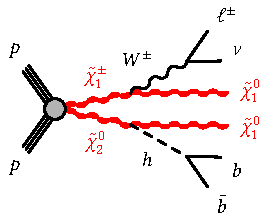
\includegraphics[width=.4\textwidth]{c1n2_wh_1lbb}
%	\caption{Diagram for the simplified model used in this work including the decays $W^\pm\rightarrow\ell^\pm\nu_\ell$ and $h\rightarrow b\bar{b}$.}\label{fig:Wh_model_full}
%\end{figure}

\begin{figure}
\floatbox[{\capbeside\thisfloatsetup{capbesideposition={right,center},capbesidewidth=0.4\textwidth}}]{figure}[\FBwidth]
{\caption{Diagram of the simplified model for $\charg\neutr$ pair production with subsequent decays into $\charg\rightarrow W^\pm\lsp \to \ell^\pm\nu_\ell\lsp$ and $\neutr\rightarrow h\lsp \to b\bar{b}\lsp$, resulting in a final state with a lepton, multiple jets and $\etmiss$.}\label{fig:Wh_model_full}}
{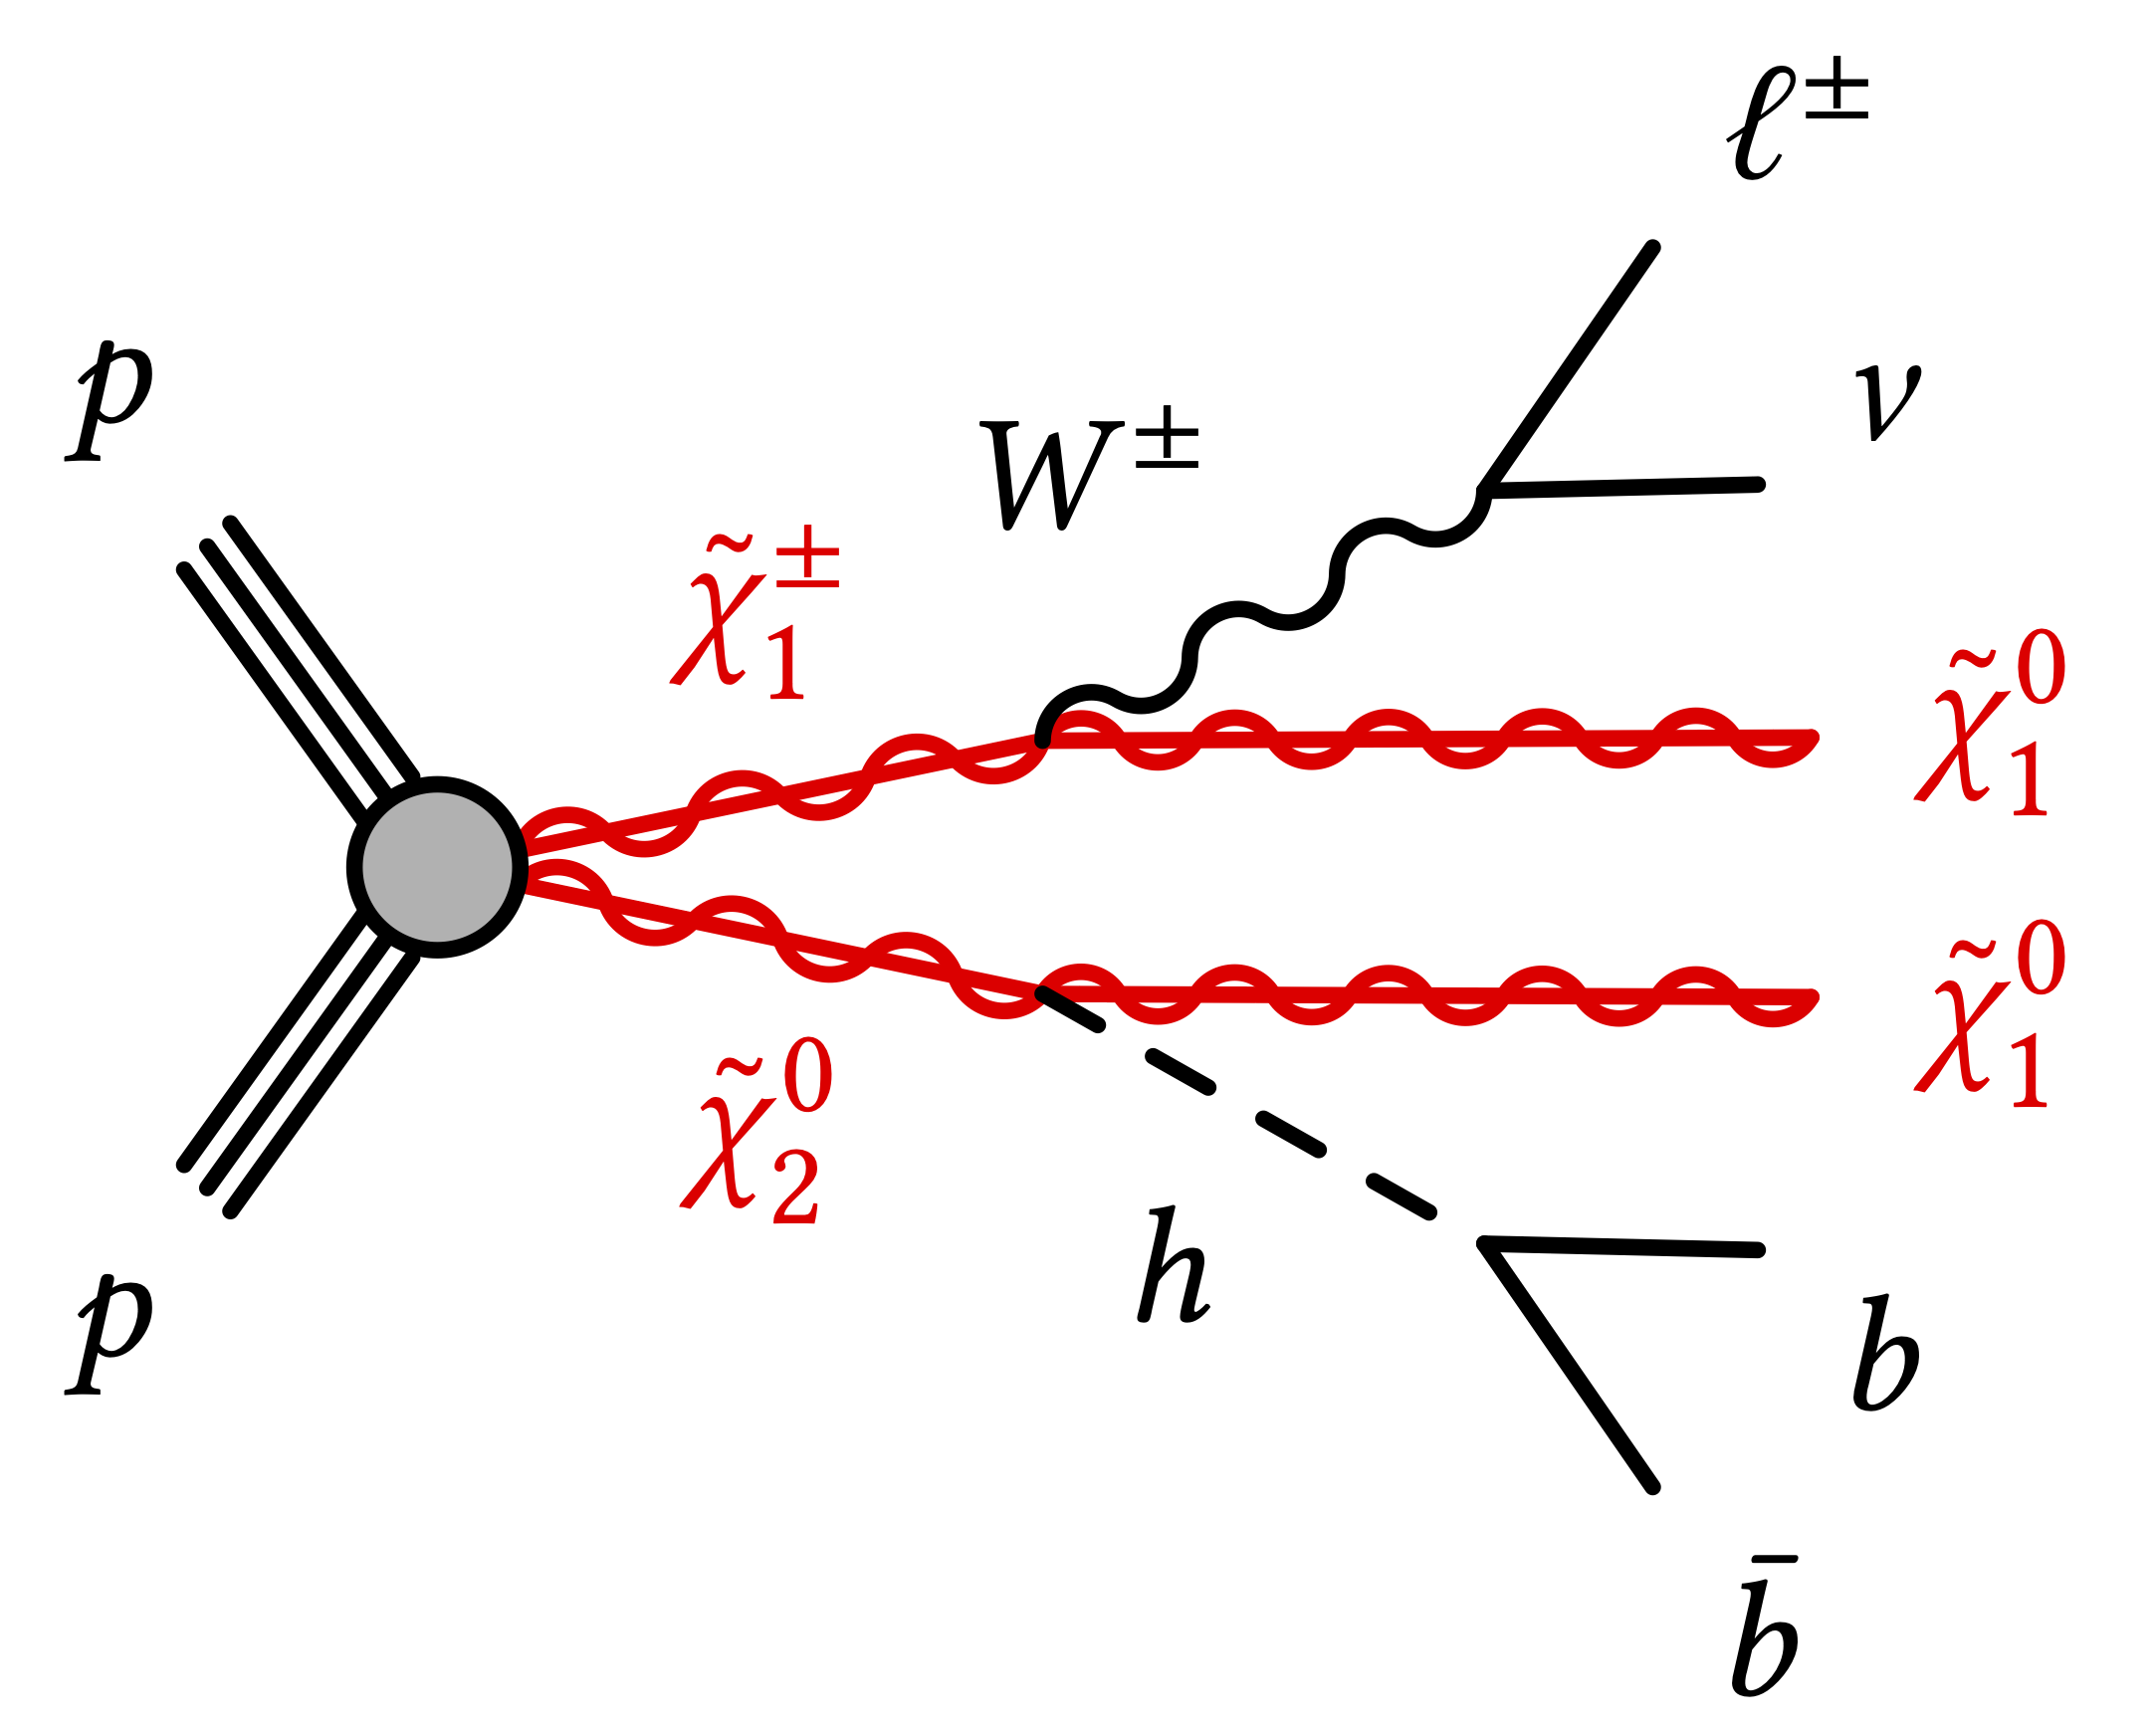
\includegraphics[width=0.35\textwidth]{c1n2_wh_1lbb.png}}
\end{figure}

\section{Standard Model backgrounds}

Although the requirement of exactly one lepton isolated from surrounding hadronic activity significantly reduces the contribution from \gls{qcd} multi-jet processes, numerous other \gls{sm} processes can still result in final states with an isolated lepton, multiple jets and missing transverse momentum.
Background sources are generally classified into \textit{reducible} and \textit{irreducible} backgrounds. Irreducible backgrounds, on the one hand, are processes with a physical phase space indistinguishable from the final state of the signal process in question. Reducible backgrounds, on the other hand, result from partially misreconstructed processes as well as mismeasurements.
Examples of reducible processes are events where a lepton originates from a \gls{hf} decay, photon conversions or misreconstructed jets. \gls{sm} processes that result in final states with an isolated electron or muon, multiple jets and missing transverse momentum typically involve a $W$ boson decaying into a lepton--neutrino pair (a so-called \textit{leptonic decay}).
The neutrino will contribute to the total missing transverse momentum in the event, while additional jets can appear in the final state through, for example, \gls{qcd} radiation.

By far the largest \gls{sm} background contribution relevant for this search stems from the production of top quarks, predominantly occurring as top quark pair production ($\ttbar$), where both top quarks decay into a $W$ boson and a $b$ quark. Final states with an isolated lepton can occur through leptonic decay of one of the $W$ bosons.
\Cref{fig:ttbar} shows a diagram of an exemplary decay of a $\ttbar$ system into a final state with a lepton, multiple jets (two of which originate from \textit{b} quarks) and missing transverse momentum.
In addition to $\ttbar$, single top production (through \textit{s}-channel, \textit{t}-channel or \textit{tW}-channel processes) can also result in similar final states as the \gls{susy} signal and thus constitutes a significant \gls{sm} background process.
An exemplary decay into a final state relevant for this search is shown in~\cref{fig:singletop}.

Apart from processes involving top quarks, the production of a $W$ boson in association with multiple jets ($\wjets$) is the third major background considered in the \onelepton search.
If the $W$ boson undergoes a leptonic decay and two of the produced jets are tagged as originating from $b$ quarks (with a procedure introduced in \cref{sec:flavour_tagging}), the signature of this process can be similar to that of signal events.
An exemplary diagram for a $\wjets$ event is illustrated in~\cref{fig:wjets}.

Production of multiple vector bosons $V$ ($=W,Z$), although not a dominant background due to low cross sections, can still result in the same final state as the signal process.
In the following, diboson ($VV$) and multiboson ($VVV$) processes are considered.

Other \gls{sm} backgrounds with small contributions in the phase spaces targeted by the search include $Z$ boson production in association with multiple jets ($Z+\mathrm{jets}$), $\ttbar$ production in association with a vector boson $V$ ($\ttbar+V$), as well as various processes involving Higgs bosons.
$Z+\mathrm{jets}$ only plays a minor role, as the only irreducible component originates from $Z(\rightarrow\tau\tau)+\mathrm{jets}$ processes, where one $\tau$-lepton undergoes a leptonic decay while the other one decays \textit{hadronically}, \ie involving a $W$ boson decaying into a pair of quarks.
Production of $\ttbar+V$ has a similar topology as ordinary $\ttbar$ processes, but with lower cross section and additional objects in the final state. This background therefore only plays a minor role in the analysis.
Higgs processes considered in the following include single Higgs production through \gls{vbf} or \gls{ggf} as well as Higgs production in association with a vector boson ($h+V$) or a top quark pair ($h+\ttbar$).
In the following, all minor backgrounds are grouped together, and collectively labelled as \textit{other} backgrounds. 
As \gls{qcd} multi-jet processes have been shown to play a negligible role in all selections relevant to this search, no estimation for \gls{qcd} contribution is considered in the following~\cite{SUSY-2019-08}.

\begin{figure}
	\centering
	\begin{subfigure}[b]{0.3\linewidth}
		\centering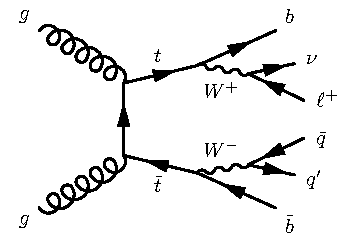
\includegraphics[width=\textwidth]{ttbar}
		\caption{\label{fig:ttbar}}
	\end{subfigure}\quad
		\begin{subfigure}[b]{0.3\linewidth}
		\centering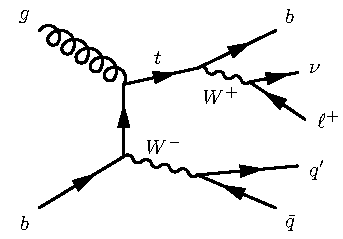
\includegraphics[width=\textwidth]{singletop}
		\caption{\label{fig:singletop}}
	\end{subfigure}\quad
	\begin{subfigure}[b]{0.3\linewidth}
		\centering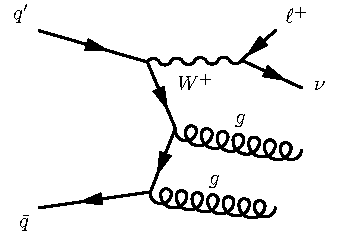
\includegraphics[width=\textwidth]{wjets}
		\caption{\label{fig:wjets}}
	\end{subfigure}
%	\begin{subfigure}[b]{0.25\linewidth}
%		\centering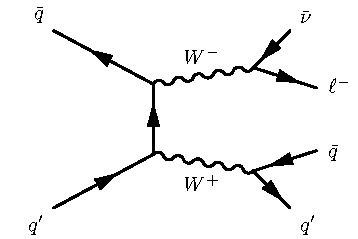
\includegraphics[width=\textwidth]{diboson}
%		\caption{\label{fig:diboson}}
%	\end{subfigure}
	\caption{Exemplary Feynman diagrams showing the dominant processes \subref{fig:ttbar} $t\bar{t}$, \subref{fig:singletop} single top and \subref{fig:wjets} $W+\textrm{jets}$ production with subsequent decays.}
	\label{fig:sm_backgrounds_feynman}
\end{figure}


\section{Monte Carlo datasets}

\Cref{tab:mc_generators} summarises all \gls{mc} generators and software versions executed during generation of the simulated events used in the following. While a brief overview on \gls{mc} \textit{weights} and the \gls{mc} datasets used is given in the following, further details are provided in the relevant ATLAS simulation notes~\cite{ATL-PHYS-PUB-2018-009,ATL-PHYS-PUB-2016-005,ATL-PHYS-PUB-2017-006,ATL-PHYS-PUB-2017-005}.

\subsection{Monte Carlo weights}\label{sec:mc_weights}

In general, \gls{mc} events can have weights that need to be considered when normalising and scaling processes to a given integrated luminosity.
Weights originate, for example, directly from the generator when including \gls{nlo} corrections in the simulation.
Another source of weights can be filtered \gls{mc} datasets, generated with specific selections in order to increase event statistics in specific regions of phase space.
Weights also arise from experimental corrections, and are, for example, used to scale efficiencies in \gls{mc} to those measured in data. Finally, reweighting of \gls{mc} events is also used to correct the \gls{mc} \textit{pile-up profile}, \ie the distribution of the mean number of inelastic $pp$ collisions per bunch crossing, such that it matches the one measured in data.
This is necessary because the \gls{mc} simulated events used herein were largely already generated before the full Run~2 dataset was recorded, and therefore before the full pile-up profile in data was known.

To obtain an event rate estimate for a given integrated luminosity, instead of the raw number of generated MC events, the sum of event weights \textit{w}, scaled to the desired integrated luminosity $L$ and total cross section $\sigma$ has to be used,
\begin{equation}
	N_\mathrm{est} =\frac{\sigma L}{\sum_{i\in\mathcal{G}}w_i} \sum_{j\in\mathcal{S}}w_j,
\end{equation}
where $i$ runs over the set of generated events $\mathcal{G}$, while $j$ runs over the set of selected events $\mathcal{S}$. The statistical uncertainty on the event rate estimate $N_\mathrm{est}$, due to the finite size of the \gls{mc} datasets, is then given by
 \begin{equation}
	\upDelta N_\mathrm{est} = \sqrt{\sum_{j\in\mathcal{S}}w_j^2}.
\end{equation}

\subsection{Signal datasets}\label{sec:signal_samples}

The $\charg\neutr$ pair production signal datasets were generated at \gls{lo} using \textsc{MadGraph5\_aMC@NLO} 2.6.2 \cite{MGaMCNLO:2014hca,Frederix:2012ps} with up to two additional partons in the matrix element. The NNPDF 2.3 LO \gls{PDF} set~\cite{Ball:2012cx} was used for calculating the hard scatter matrix elements.
\textsc{MadGraph5\_aMC@NLO} is interfaced with \textsc{Pythia8}~\cite{Pythia8:2007gs} for the parton shower, hadronisation and underlying event, using the A14 set of tuned parameters~\cite{ATL-PHYS-PUB-2014-021}. The CKKW-L~\cite{Lonnblad:2011xx} scheme for matching the parton showers to the matrix elements was used with a nominal merging scale of $\SI{30}{\GeV}$.
For modelling the decays of heavy flavour quarks, \textsc{EvtGen} v1.6~\cite{Lange:2001uf} is used. 

As the $\charg$/$\neutr$ and $\lsp$ masses are free parameters of the signal model, they are systematically varied, resulting in the set of 125 distinct signal models shown in~\cref{fig:signalgrid}, distributed in the two-dimensional grid spanned by the two mass parameters.
The generated signal grid covers $\charg$/$\neutr$ masses from $\SI{150}{\GeV}$ to $\SI{1}{\TeV}$ and $\lsp$ masses from $\SI{0}{\GeV}$ to $\SI{400}{\GeV}$, avoiding the kinematically forbidden region with \mbox{$m(\charg$/$\neutr) < m(\lsp) + m(h)$} that does not allow for production of on-shell Higgs bosons.

\gls{mc} datasets of signal models well within the expected sensitivity range of the analysis, \ie with relatively low $\charg$/$\neutr$ and $\lsp$ masses, are generated using the \textsc{ATLFAST-II}~\cite{Aad:2010ah} detector simulation. The full detector simulation using \textsc{Geant4}~\cite{geant:2002hh} is used for the remaining model points for maximum accuracy in the parameter space relevant to the expected sensitivity. So as to account for pile-up effects, all signal datasets are overlaid with simulated minimum bias events generated using \textsc{Pythia8} and the A3 tune~\cite{ATL-PHYS-PUB-2016-017}, and reweighted to match the pile-up distribution measured in data. 

The cross sections for electroweakino pair production have been calculated using \mbox{\textsc{Resummino}}~\cite{Fuks:2013vua} at \gls{nlo} in the strong coupling constant and including \gls{nll} terms in the soft gluon resummation~\cite{Fiaschi:2018hgm,Fuks:2012qx}.

\subsection{Background datasets}

Top quark pair production and single top processes were generated using \textsc{Powheg-Box} v2~\cite{PowhegBox:2010xd}, implementing the \textsc{Powheg} method~\cite{Powheg1,Powheg2} for merging \gls{nlo} matrix elements with the parton showers without resorting to negative event weights\footnote{It is, in general, desirable to avoid negative \gls{mc} weights when generating \gls{mc} events, as they not only dilute the statistical power of the dataset generated, but also need to be processed through the time-consuming detector simulation.}.
The parton showering, hadronisation and underlying event were simulated using \textsc{Pythia8}. Production of $\ttbar+V$ is generated using \textsc{MadGraph5\_aMC@NLO} 2.3.3, interfaced with \textsc{Pythia8} for the parton showering. 
$W/Z+\mathrm{jets}$ processes are simulated using \textsc{Sherpa} 2.2.1~\cite{Gleisberg:2008ta,Bothmann:2019yzt}, allowing for up to two (four) additional parton emissions at NLO (LO) accuracy. 
%The CKKW scheme~\cite{Hoeche:2009rj,Catani:2001cc}, extended to NLO accuracy~\cite{Hoeche:2012yf}, is used for matching and merging the matrix elements and parton showers. 
For diboson and multiboson  processes both \textsc{Sherpa} 2.2.1 and 2.2.2 were used. 
All Higgs processes are simulated using \textsc{Powheg-Box} v2 for the matrix element calculations and \textsc{Pythia8} for the parton showers, underlying event and hadronisation. 
%While the generation of $h+\ttbar$ uses the A14 tune and the NNPDF2.3LO set, $h+V$ and single Higgs production are simulated using the NNPDF 3.0 NNLO set and the AZNLO~\cite{ATL-PHYS-PUB-2013-017} set of tuned generator parameters.

For maximum modelling accuracy, the detector simulation for all \gls{mc} background datasets was performed using the full detector simulation based on \textsc{Geant4}. Except for the \gls{mc} datasets generated using \textsc{Sherpa}, all background datasets use \textsc{EvtGen}~\cite{Lange:2001uf} to improve the modelling of heavy flavour decays and \textit{b}-tagging efficiency. Similar to the signal models, pile-up effects are taken into account by overlaying all background datasets with simulated minimum bias events generated with \textsc{Pythia8} using the NNPDF 2.3 LO \gls{PDF} set~\cite{Ball:2012cx} and the A3 tune~\cite{ATL-PHYS-PUB-2016-017} of parameters. 

\Cref{tab:mc_generators} also lists the accuracies up to which the theoretical cross sections, used to normalise the event rates to a given integrated luminosity, have been calculated. The normalisations of the main \gls{sm} backgrounds $\ttbar$, single top and $\wjets$ are derived from data in the final statistical evaluation, therefore their theoretical cross sections are only used during the development of the analysis strategy.

\begin{table}
	\centering
	\setlength\heavyrulewidth{0.2ex}
	\small
	\caption{Overview of the configuration of \gls{mc} generators used for simulating the various \gls{susy} signal and \gls{sm} background processes. While two different \gls{PDF} sets are typically used for matrix element calculations and parton showering, only the former one is given in the table. The `tune' refers to the set of tuned parameters used for parton showering and hadronisation. For conciseness, \textsc{MadGraph5\_aMC@NLO} is abbreviated as \textsc{MG5\_aMC@NLO}.}
	\resizebox{\textwidth}{!}{\begin{tabular} {llllll}
	\toprule
	Process & Matrix element & Parton shower & PDF set & Cross section & Tune\\ 
	\midrule
	Signal & \textsc{MG5\_aMC@NLO} 2.6.2 & \textsc{Pythia} 8.230 & NNPDF 2.3 LO~\cite{Ball:2012cx} & NLO+NLL~\cite{Fuks:2013vua,Fiaschi:2018hgm,Fuks:2012qx} & A14~\cite{ATL-PHYS-PUB-2014-021} \\
	\midrule	
	$\ttbar$ & \textsc{Powheg-Box} v2 & \textsc{Pythia} 8.230 & NNPDF 3.0 NLO~\cite{Ball:2014uwa} & NNLO+NNLL~\cite{Czakon:2011xx,Cacciari:2011hy} & A14 \\
	$t$ (s-channel) & \textsc{Powheg-Box} v2 & \textsc{Pythia} 8.230 & NNPDF 3.0 NLO & NLO~\cite{Kant:2014oha} & A14 \\
	$t$ (t-channel) & \textsc{Powheg-Box} v2 & \textsc{Pythia} 8.230 & NNPDF 3.0 NLO & NLO~\cite{Kant:2014oha} & A14 \\
	$t+W$ & \textsc{Powheg-Box} v2 & \textsc{Pythia} 8.230 & NNPDF 3.0 NLO & NNLO~\cite{Kant:2014oha,Kidonakis:2010ux} & A14 \\
	$\ttbar + V$ & \textsc{MG5\_aMC@NLO} 2.3.3 & \textsc{Pythia} 8.210 & NNPDF 3.0 NLO & NLO~\cite{Campbell:2012dh,Lazopoulos:2008de} & A14 \\
	\midrule
	$V+\mathrm{jets}$ & \multicolumn{2}{c}{\textsc{Sherpa} 2.2.1} & NNPDF 3.0 NNLO~\cite{Ball:2014uwa} & NNLO~\cite{Gavin:2010az} & \textsc{Sherpa} default \\
	$VV$ & \multicolumn{2}{c}{\textsc{Sherpa} 2.2.1/2.2.2} & NNPDF 3.0 NNLO & NLO~\cite{ATL-PHYS-PUB-2017-005} & \textsc{Sherpa} default\\
	$VVV$ & \multicolumn{2}{c}{\textsc{Sherpa} 2.2.1/2.2.2} & NNPDF 3.0 NNLO & NLO~\cite{ATL-PHYS-PUB-2017-005} & \textsc{Sherpa} default\\
	\midrule
	$h+\ttbar$ & \textsc{Powheg-Box} v2 & \textsc{Pythia} 8.230 & NNPDF 3.0 NLO & NLO~\cite{deFlorian:2016spz} & A14 \\
	$h+V$ & \textsc{Powheg-Box} v2 & \textsc{Pythia} 8.212 & NNPDF 3.0 NNLO & NNLO+NLO~\cite{deFlorian:2016spz} & AZNLO~\cite{ATL-PHYS-PUB-2013-017} \\
	\textit{h (ggF)} & \textsc{Powheg-Box} v2 & \textsc{Pythia} 8.212 & NNPDF 3.0 NNLO & N$^3$LO+N$^3$LL~\cite{deFlorian:2016spz} & AZNLO \\
	\textit{h (VBF)} & \textsc{Powheg-Box} v2 & \textsc{Pythia} 8.212 & NNPDF 3.0 NNLO & NNLO+NLO~\cite{deFlorian:2016spz} & AZNLO \\
	\bottomrule
	\end{tabular}}\vspace{2mm}
	\label{tab:mc_generators}   
\end{table}

\section{Object definitions}\label{sec:object_definitions}

The reconstruction and identification of physics objects\footnote{The term \textit{physics objects} denotes the objects reconstructed from the measured detector signals, rather than the actual physical particle(s) of interest traversing the detector. As such, a reconstructed electron, for example, may not necessarily correspond to a real, physical electron but only has a certain probability to be a true electron.} requires the combination of data from multiple detector components.
Due to finite detector resolutions, and the considerable amount of particles produced in each collision, this process does not always work without flaws.
Sometimes, objects are falsely reconstructed or not reconstructed at all. In order to minimise reconstruction errors, different identification and reconstruction criteria are introduced for each physics object category. Electrons and muons are categorised into \textit{baseline} and \textit{signal} objects.
Baseline objects have a smaller purity but a higher acceptance which is useful for, \eg, the reconstruction of the missing transverse momentum. Stricter identification and isolation criteria are required for signal objects, resulting in lower acceptances but also lower probability of reconstruction errors.
In the following, mostly signal-type objects are used as the physics objects. \Cref{tab:objdef} provides a summary of the object definitions introduced in the ensuing sections.

\subsection{Tracks and vertices}\label{sec:reco_tracks}

The reconstruction of tracks of charged particles starts with the formation of clusters from raw data recorded in the Pixel and \gls{sct} detectors.
Clusters are formed by grouping together adjacent pixels and strips with energy deposits above a certain threshold and are subsequently used to create three-dimensional space-points, representing the points where charged particles traversed the active \gls{id} material~\cite{PERF-2015-08}.
Sets of three space-points form track seeds that serve as inputs for a combinatorial Kalman filtering technique~\cite{Fruhwirth:178627} that includes additional space-points from the remaining pixel and \gls{sct} layers to extend the preliminary trajectory.
A $\chi^2$ track fit is performed at each step of the extension.
Where seeds can be extended by more than one compatible space-point in a given layer, multiple track candidates are formed.
Ambiguities between candidates are resolved by assigning them a score, taking into account basic track properties like the $\chi^2$ of the track fit and its associated $\pt$~\cite{PERF-2015-08}.
The ambiguity solver requires track candidates to contain a minimum of 7 pixel and \gls{sct} clusters, to have a maximum of one shared pixel cluster and two shared \gls{sct} clusters on the same layer and to have no more than two holes\footnote{Holes are intersections of the track trajectory with sensitive detector material not containing a cluster.} of which only one is allowed to be in the pixel detector.
Track candidates also need to have $\pt > \SI{400}{\MeV}$, $\vert\eta\vert < 2.5$ and have longitudinal ($z_0$) and transversal ($d_0$) impact parameters with respect to their associated vertex satisfying $\vert z_0 \sin\theta \vert < \SI{3.0}{\milli\meter}$ and $\vert d_0 \vert < \SI{2.0}{\milli\meter}$, where $\theta$ is the polar angle of the track~\cite{PERF-2015-08}.
Track candidates surviving the ambiguity solver are extended by compatible hits in the \gls{trt}~\cite{Cornelissen:1176900} and are subject to a global high-resolution track fit before being added to the final track collection~\cite{PERF-2015-08}.

Vertex reconstruction uses a selection of tracks satisfying a set of quality requirements~\cite{ATL-PHYS-PUB-2015-026} in order to fit the best vertex position through a procedure iteratively down-weighting less compatible tracks~\cite{PERF-2015-01}. Once the vertex position has been determined, incompatible tracks with small weights are removed and can be reused for the reconstruction of additional vertices~\cite{PERF-2015-01}.
All reconstructed vertices with at least two associated tracks are kept as valid primary vertex candidates. In events with multiple candidates, the primary vertex is defined to be the one with the highest $\sum \pt^2$ of its associated tracks.

\subsection{Electrons and Photons}\label{sec:reco_electrons}

Electron and photon candidates are reconstructed from energy deposits in topologically connected cells in the electromagnetic and hadronic calorimeters.
The reconstruction algorithm starts with the preparation of energy deposits into so-called \textit{topo-clusters}~\cite{PERF-2014-07}.
These are formed by calorimeter cells containing energy deposits above a certain noise threshold, so-called \textit{seed} cells, including their neighbouring cells which, in turn, can also act as seed cells.
All cell signals are measured at the electromagnetic scale, assuming that energy deposits stem only from electromagnetic interactions.
Although the topo-clustering algorithm starts with cells from both calorimeters, only energies from cells in the \gls{em} calorimeter are used in the subsequent electron and photon reconstruction steps~\cite{EGAM-2018-01}.
Using only \gls{em} topo-clusters with a certain threshold ratio of the \gls{em} energy to the total cluster energy significantly reduces contamination from pile-up clusters~\cite{EGAM-2018-01}.
Next, the \gls{em} topo-clusters are loosely matched to \gls{id} tracks which are subsequently re-fitted in order to account for energy losses through bremsstrahlung~\cite{EGAM-2018-01}.
Vertices from photon conversions are reconstructed from tracks matched to fixed-size clusters~\cite{PERF-2017-02} and also matched to the \gls{em} topo-clusters.
In the final step of the reconstruction algorithm, \gls{em} topo-clusters are sorted according to descending $E_{\mathrm{T}}$ and tested as seed clusters for dynamic, variable-size \textit{superclusters}, with different seed requirements for electrons and photons~\cite{EGAM-2018-01}.
Clusters near seed candidates can be added as satellite cluster candidates, originating for example from bremsstrahlung. The supercluster technique allows to dynamically change the cluster size as needed to recover energy losses from bremsstrahlung or photon conversions~\cite{EGAM-2018-01}.
Electrons are finally built from superclusters with matched tracks.
While converted photons are built from supercluster and matched conversion vertices, unconverted photons are constructed using superclusters not matched to any electron tracks or conversion vertices.
The energies of both electrons and photons are calibrated using $Z\rightarrow ee$ decays~\cite{EGAM-2018-01}.

The identification of prompt electrons relies on a likelihood discriminant built from quantities measured in the \gls{id} and calorimeters~\cite{PERF-2017-01}.
The quantities are chosen according to their ability to discriminate prompt isolated electrons from non-prompt leptons originating in, \eg, \gls{hf} decays, from photon conversions or from jets.
They include the properties of the electron track, the shape of the \gls{em} shower and the quality of the match between the electron track and the calorimeter clusters~\cite{PERF-2017-01}.
Photon identification, on the other hand, relies on a cut-based\footnote{The term \textit{cut} refers to simple upper or lower requirement on a measurable quantity.} selection exploiting the shape of the \gls{em} shower~\cite{EGAM-2018-01}.

In the \onelepton search, electrons are required to satisfy $\pt > \SI{7}{GeV}$ and $\vert\eta\vert<2.47$.
Baseline electrons are identified using the \textit{LooseAndBLayer}~\cite{PERF-2017-01} requirement on the identification likelihood, requiring a hit in the innermost layer of the pixel detector, at least two additional hits in the remaining pixel layers and seven hits in the pixel and \gls{sct} detectors combined.
In addition, the longitudinal impact parameter $z_0$ of baseline electrons needs to satisfy $\upDelta z_0\sin\theta < \SI{0.5}{\milli\meter}$ with respect to the primary vertex.
The \textit{LooseAndBLayer} identification yields an average efficiency of about 93\%, increasing from low to high electron $E_\mathrm{T}$.
Signal electrons are a subset of baseline electrons and need to satisfy the \textit{Tight}~\cite{PERF-2017-01} likelihood identification, yielding an efficiency of 80\% for prompt electrons with $E_\mathrm{T}=\SI{40}{\GeV}$~\cite{PERF-2017-01}.
In addition to the longitudinal impact parameter, signal leptons also need to satisfy $d_0/\sigma_{d_0} < 5$, where the transverse impact parameter $d_0$ and its uncertainty $\sigma_{d_0}$ are measured with respect to the beam line. 

Finally, electrons need to be \textit{isolated}, meaning that their vicinity must be clear of additional significant detector activity.
Requiring electrons to be isolated prevents the selection of non-prompt electrons originating from, \eg, \gls{hf} decays or misidentifications of light hadrons.
Isolation is quantified using two observables, one relying on tracking information and the other one using calorimeter data. The tracking based isolation variable, $p_{\mathrm{T}}^{\mathrm{var20}}$, is the sum of all track momenta above $\SI{1}{\GeV}$ (excluding the electron track itself) in a cone around the electron~\cite{EGAM-2018-01}.
The size of the cone is chosen to be $\upDelta R = \min (\SI{10}{\GeV}/\pt,0.2)$, \ie is shrinking with increasing transverse momentum of the electron.
The calorimeter based variable $E_{\mathrm{T}}^{\mathrm{cone20}}$ corresponds to the sum of the transverse energies in topo-clusters (excluding the electrons itself and after correcting for pile-up effects) in a cone with $\upDelta R = 0.2$ around the electrons~\cite{EGAM-2018-01}.
Both baseline and signal electrons are required to satisfy the \textit{Loose}~\cite{EGAM-2018-01} working point, corresponding to the requirements $p_{\mathrm{T}}^{\mathrm{var20}}/\pt < 0.2$ and $E_{\mathrm{T}}^{\mathrm{cone20}} < 0.15$.
In order to improve the rejection of non-prompt electrons at high transverse momenta, electrons with $\pt >\SI{200}{\GeV}$ need to satisfy the \textit{HighPtCaloOnly} working point, applying the tighter requirement $E_{\mathrm{T}}^{\mathrm{cone20}} < \max (0.015\cdot\pt,\SI{3.5}{\GeV})$. 

Photons are required to have $\pt > \SI{13}{GeV}$ and $\vert\eta\vert<2.37$ and need to satisfy the \textit{Tight}~\cite{EGAM-2018-01} identification and \textit{FixedCutTight}~\cite{EGAM-2018-01} isolation requirements.
In this analysis, photons are only used in the calculation of the missing transverse momentum.

\subsection{Muons}\label{sec:reco_muon}

The reconstruction of muons uses primarily data from the \gls{id} and \gls{ms} and is based on the minimum ionising nature of muons. Muon candidates are independently reconstructed in the \gls{id} and the \gls{ms} as muon tracks and subsequently combined to a muon candidate that can be used by physics analyses~\cite{PERF-2015-10,Aad:2020gmm}.
The track reconstruction in the \gls{id} follows the same procedure used for other charged-particle tracks, described in \cref{sec:reco_tracks}.
In the \gls{ms}, the muon track reconstruction starts with the identification of short, straight-line track segments. Segments from different \gls{ms} layers are combined into preliminary muon track candidates if they are loosely compatible with the \gls{ip} and match a first-order approximation of the parabolic trajectory describing the muon track in the magnetic field~\cite{Aad:2020gmm}.
Track candidates are then passed through a global $\chi^2$ fit, taking into account possible \gls{ms} chamber misalignments as well as interactions with the detector material~\cite{Aad:2020gmm}.
In order to increase the reconstruction performance, \gls{ms} muon tracks are subsequently combined with the \gls{id} tracks using five different reconstruction strategies, described in detail in \reference\cite{Aad:2020gmm}.
Only two of these strategies are relevant for this analysis:
\begin{itemize}
	\item \textit{combined muons}, formed by combining the \gls{id} and \gls{ms} tracks through a global fit, taking into account the energy loss in the calorimeters. An \textit{outside-in} approach is employed, reconstructing muons first in the \gls{ms} before performing an inward extrapolation and match to an \gls{id} track.
	\item \textit{\gls{ms} extrapolated muons}, built using \gls{ms} muon tracks only, but extrapolating the tracks back to the \gls{ip} and requiring them to be loosely compatible with the \gls{ip}. Extrapolated muons are mainly used for providing acceptance in the region $2.5 < \vert\eta\vert < 2.7$, which is beyond the coverage provided by the \gls{id}.
\end{itemize}
After resolving the overlaps between the different muon types, the muon objects used for physics analysis are subject to a momentum calibration using data from $J/\Psi\rightarrow\mu\mu$ and $Z\rightarrow\mu\mu$ decays~\cite{Aad:2020gmm}.

Identification of muons is performed using a set of quality requirements, designed to suppress non-prompt muons originating from pion and kaon decays while allowing a robust momentum measurement.
Muons in this analysis are built using combined and extrapolated muons that satisfy the \textit{Medium} identification requirements~\cite{PERF-2015-10}.
This requires combined muons to have at least three hits in at least two \gls{mdt} layers---except for the region with $\vert\eta\vert < 0.1$, where a single \gls{mdt} layer is enough, as long as there is no more than one \gls{mdt} hole layer~\cite{Aad:2020gmm}.
Extrapolated muons need to have at least three hits in at least three \gls{mdt} and \gls{csc} layers~\cite{Aad:2020gmm}.
In addition, all muons are required to have a significance of the ratio of the measured charge and momentum satisfying $\sigma(q/p) < 7$.
The identification of muons with the \textit{Medium} identification working point is evaluated in $J/\Psi\rightarrow\mu\mu$ and $Z\rightarrow\mu\mu$ events and yields an efficiency of more than 98\% for muons with $\pt > \SI{6}{\GeV}$ and $\vert\eta\vert < 2.5$~\cite{Aad:2020gmm}.
The light-hadron rejection rate, measured in simulated $\ttbar$ events, is roughly 98 for low-$\pt$ muons with $\pt < \SI{20}{\GeV}$, and increases to 830 for muons with $\pt > \SI{100}{\GeV}$~\cite{Aad:2020gmm}.

Baseline muons in this analysis need to satisfy $\pt > \SI{6}{\GeV}$ and be within $\vert\eta\vert < 2.7$. Furthermore, the longitudinal impact parameter of baseline muons with respect to the primary vertex is required to be $\upDelta z_0\sin\theta < \SI{0.5}{\milli\meter}$.
Signal muons additionally need to be within $\vert\eta\vert < 2.5$ and have a transverse impact parameter satisfying $d_0/\sigma_{d_0} < 3$. Similar to electrons, muons also have to be isolated, using the same variables used for electron isolation.
Both signal and baseline muons need to conform to the \textit{Loose}~\cite{Aad:2020gmm} working point, requiring $p_{\mathrm{T}}^{\mathrm{var20}}/\pt < 0.3$ and $E_{\mathrm{T}}^{\mathrm{cone20}} < 0.15$.
The \textit{Loose} isolation working point yields an efficiency quickly increasing from 86\% for muons with $\SI{5}{\GeV} < \pt < \SI{20}{\GeV}$ to 97\% for muons with $\SI{20}{\GeV} < \pt < \SI{100}{\GeV}$.
Muons with $\pt > \SI{100}{\GeV}$ have an isolation efficiency of more than 99\%~\cite{Aad:2020gmm}. The rejection rate for muons from \gls{hf} decays ranges from 14 to 8 with increasing $\pt$ in the range relevant for the \onelepton search~\cite{Aad:2020gmm}.

\subsection{Jets}\label{sec:jets}

Jets are reconstructed using the anti-$k_t$ algorithm~\cite{Cacciari:2008gp}, implemented in the \textsc{FastJet}~\cite{Fastjet,Cacciari:2006sm} package.
A radius parameter of $R=0.4$ is used for all jets considered in the following. The inputs to the anti-$k_t$ algorithm are topo-clusters~\cite{Aad:2020flx}, built at the \gls{em} scale using the procedure introduced in~\cref{sec:reco_electrons}.
Tracks with $\pt > \SI{500}{\MeV}$ and an association to the primary vertex are assigned to jets using \textit{ghost association}~\cite{Cacciari:2007fd}, a method treating them as particles with infinitesimal momentum such that the properties of the calorimeter-based jets are not changed. 

Reconstructed jets undergo a \gls{jes} calibration, correcting the four-momentum and scaling the energy and mass~\cite{Aad:2020flx}.
In a first step, energy contributions from in-time and out-of-time pile-up are removed using a data-driven jet-by-jet approach based on the jet area $A$ and pile-up $\pt$ density $\rho = p_\mathrm{T}/A$. The jet area is determined by the relative number of ghost particles (added uniformly in solid angle to the event prior to jet clustering) associated to the jet after clustering. 
Additionally, a residual correction derived from \gls{mc} simulation is applied, parameterised in the number of mean interactions per bunch crossing and the number of reconstructed primary vertices~\cite{Aad:2020flx,Cacciari:2007fd}.
The reconstructed jet four-momentum is corrected to the particle-level energy scale through an absolute \gls{jes} and $\eta$ calibration.
In order to reduce the dependence of the jet response (\ie the ratio between the measured jet energy and the true jet energy) on the flavour and energy distribution of its constituents, a series of multiplicative corrections is applied~\cite{PERF-2011-03}.
These improve the \gls{jer} and are based on data from the calorimeters, jet-related tracking information, as well as \gls{ms} information.
Differences between the jet response in data and \gls{mc} simulation, caused by imperfect detector and physics simulations, are corrected using so-called \textit{in situ} calibrations~\cite{Aad:2020flx}.
The jet response in data and \gls{mc} simulations is measured separately, allowing to derive a correction factor that is applied on data.
Similarly to the \gls{jes}, the \gls{jer} is also calibrated. Its calibration is performed using $\pt$-asymmetry measurements in dijet events~\cite{PERF-2014-02}.

Even after the subtraction of pile-up effects, some pile-up jets still remain. The \gls{jvt}~\cite{PERF-2014-03}, a multivariate discriminant, is used to suppress pile-up jets.
It is based on variables that describe the fraction of the total jet momentum corresponding to tracks associated to the primary vertex.
In the \onelepton search, jets with $\pt < \SI{120}{\GeV}$ and $\vert\eta\vert < 2.5$ need to be associated to the primary vertex using the \textit{medium}~\cite{Aad:2020flx} working point, achieving an average 92\% efficiency for jets originating from the hard scatter interaction.

Baseline jets in this analysis are required to have $\pt > \SI{20}{\GeV}$ and $\vert\eta\vert < 4.5$. Analysis variables are built using signal-level jets with $\pt > \SI{30}{\GeV}$ and $\vert\eta\vert < 2.8$.

\subsection{Flavour tagging}\label{sec:flavour_tagging}

As can be seen through the \gls{ckm} matrix, \textit{b} quarks primarily decay through $b\rightarrow W c$.
However, due to the small coupling constant proportional to the corresponding \gls{ckm} matrix element $V_{cb}$ (corresponding to the $b \leftrightarrow c $ transition), \textit{B} hadrons have a relatively long lifetime of the order of $\SI{1.5}{\pico\second}$ ($\braket{c\tau} \approx \SI{450}{\micro\meter}$)~\cite{pdg2020}.
In the typical momentum ranges, \textit{B} hadrons can thus have a measurable flight length before decaying, leading to secondary vertices that are displaced from the hard-scatter primary vertex.
ATLAS uses a collection of algorithms designed to discern \gls{hf} jets containing \textit{B} hadrons from light-flavour jets by exploiting the impact parameters or reconstructing the displaced vertices.
A multivariate classifier, called \texttt{MV2}~\cite{ATL-PHYS-PUB-2017-013}, combines the outputs of the different taggers using a \gls{bdt} algorithm that is trained on simulated $\ttbar + Z'$ events. 

Due to the Higgs decay into $b$ quarks in the signal model targeted, \textit{b}-tagged jets play a crucial role in the analysis described in this work.
Baseline jets with $\vert\eta\vert < 2.5$ are used as input to the \texttt{MV2c10} \textit{b}-tagging algorithm, an implementation of the \texttt{MV2} discriminant using a \textit{c}-jet fraction of 7\% during the \gls{bdt} training~\cite{FTAG-2018-01, PERF-2016-05}.
The working point chosen for the \texttt{MV2c10} tagger achieves a \textit{b}-tagging efficiency of 77\% with rejection rates of $4.9$, $15$, and $110$ for \textit{c}-jets, $\tau$-jets and light-flavour jets, respectively, measured in simulated $\ttbar$ and dijet events~\cite{FTAG-2018-01}.

\subsection{Missing transverse momentum}

Momentum conservation in the transverse plane implies that the sum of the transverse momenta of all objects in a $pp$ collision should vanish.
Particles escaping the detector without being measured thus lead to a momentum imbalance, in the following referred to as missing transverse momentum $\makemebold{p}^{\textrm{miss}}_\textrm{T}$ with magnitude $\etmiss$.
The missing transverse momentum in each event is computed using all reconstructed objects and takes into account tracks associated to the primary vertex but not used for any reconstructed object~\cite{PERF-2016-07}, yielding
\begin{equation}
	\makemebold{p}^{\textrm{miss}}_\textrm{T} = - \sum\makemebold{p}^{e}_{\textrm{T}} - \sum\makemebold{p}^{\gamma}_{\textrm{T}} - \sum\makemebold{p}^{\mu}_{\textrm{T}} - \sum\makemebold{p}^{\mathrm{jet}}_{\textrm{T}} - \sum\makemebold{p}^{\mathrm{track}}_{\textrm{T}}.
	\label{eq:met}
\end{equation}
While terms originating from the reconstructed, calibrated objects are collectively referred to as the \textit{hard term}, the remaining track term is referred to as \textit{soft term}.
As $\tau$-leptons are not explicitly reconstructed in this analysis, no dedicated $\tau$-term is included in \cref{eq:met}. Instead, $\tau$-leptons are included in the electron, muon or jet term, depending on their decay mode and reconstruction. The computation of $\etmiss$ uses all baseline objects introduced in the previous sections. Ambiguities between objects are resolved using an overlap removal procedure~\cite{PERF-2016-07} that is separate and independent from the procedure described in \cref{sec:overlap_removal}. In order to reduce effects from pile-up, the $\etmiss$ is computed using the \textit{Tight} working point described in Ref.~\cite{ATLAS-CONF-2018-023}, excluding forward jets with $\vert\eta\vert > 2.4$ and $\pt < \SI{30}{\GeV}$.

Events without any true $\etmiss$ can have non-zero reconstructed $\etmiss$ due to residual pile-up effects, object mismeasurements or particles escaping through uninstrumented regions of the detector. Such \textit{fake} $\etmiss$ allows events without any real $\etmiss$ (\eg $Z(\rightarrow ee)+\mathrm{jets}$) to pass the event selection criteria and end up in the kinematic regions of interest, even after requiring a certain threshold value of $\etmiss$.


\begin{table}
	\centering
	\setlength\heavyrulewidth{0.2ex}
	\small
	\caption{Overview of the object definitions used. A dash `--' indicates where no requirement is made.}
	\begin{tabular} {lll}
	\toprule
	Property & Baseline type & Signal type \\ 
	\midrule
	\multicolumn{3}{c}{Electrons} \\
	\midrule
	Kinematic &  $\pt > \SI{7}{GeV}$, $\vert\eta\vert<2.47$ & $\pt > \SI{7}{GeV}$, $\vert\eta\vert<2.47$\\
	Identification &  \textit{LooseAndBLayer}~\cite{PERF-2017-01} & \textit{Tight}~\cite{PERF-2017-01} \\
	Impact parameters & $\upDelta z_0\sin\theta < \SI{0.5}{\milli\meter}$ & $\upDelta z_0\sin\theta < \SI{0.5}{\milli\meter}$, $d_0/\sigma_{d_0} < 5$ \\
	\multirow{2}*{Isolation} & \multirow{2}*{--} & \textit{Loose}~\cite{EGAM-2018-01} ($\pt \leq \SI{200}{\GeV}$) \\
	& & \textit{HighPtCaloOnly}~\cite{EGAM-2018-01} ($\pt > \SI{200}{\GeV}$) \\
	\midrule
	\multicolumn{3}{c}{Muons} \\
	\midrule
	Kinematic &  $\pt > \SI{6}{GeV}$, $\vert\eta\vert<2.7$ & $\pt > \SI{6}{GeV}$, $\vert\eta\vert<2.5$\\
	Identification &  \textit{Medium}~\cite{PERF-2015-10} & \textit{Medium}~\cite{PERF-2015-10} \\
	Impact parameters & $\upDelta z_0\sin\theta < \SI{0.5}{\milli\meter}$ & $\upDelta z_0\sin\theta < \SI{0.5}{\milli\meter}$, $d_0/\sigma_{d_0} < 3$ \\
	Isolation & -- & \textit{Loose}~\cite{Aad:2020gmm}\\
	\midrule
		\multicolumn{3}{c}{Jets} \\
	\midrule
	Kinematic &  $\pt > \SI{20}{GeV}$, $\vert\eta\vert<4.5$ & $\pt > \SI{30}{GeV}$, $\vert\eta\vert<2.8$\\
	\gls{jvt} & -- &  \textit{Medium}~\cite{Aad:2020flx}, $\pt < \SI{120}{\GeV}$, $\vert\eta\vert < 2.5$ \\
	\midrule
		\multicolumn{3}{c}{\textit{b}-jets} \\
	\midrule
	Kinematic &  $\pt > \SI{20}{GeV}$, $\vert\eta\vert<4.5$ & $\pt > \SI{30}{GeV}$, $\vert\eta\vert<2.5$\\
	\gls{jvt} & -- &  \textit{Medium}~\cite{Aad:2020flx}, $\pt < \SI{120}{\GeV}$, $\vert\eta\vert < 2.5$  \\
	\textit{b}-tagging & -- & \texttt{MV2c10}~\cite{FTAG-2018-01} with 77\% efficiency \\
	\bottomrule
	\end{tabular}\vspace{2mm}
	\label{tab:objdef}   
\end{table}

\section{Overlap removal}\label{sec:overlap_removal}

As the reconstruction procedure runs independently for each object type, it may happen that the same tracks or energy deposits in the calorimeters are used for the reconstruction of two different objects. For example, electrons are often also reconstructed as electron-seeded jets~\cite{overlapremoval:1700874}. In order to resolve ambiguities and prevent double-counting, an overlap removal procedure using the distance parameter $\upDelta R_y = \sqrt{(\upDelta y)^2+(\upDelta \phi)^2}$ is performed. The procedure sequentially runs the following steps on baseline objects, with only surviving objects participating in subsequent steps:
\begin{enumerate}
	\item Electrons sharing an \gls{id} track with a muon are removed, preventing duplication of muons as electrons via bremsstrahlung with subsequent photon conversion~\cite{overlapremoval:1700874}.
	\item Jets within $\upDelta R_y < 0.2$ of an electron are rejected, preventing the pure duplication of electrons as electron-seeded jets~\cite{overlapremoval:1700874}.
	\item Electrons overlapping with remaining jets within $\upDelta R_y = \min (0.4, 0.04+\SI{10}{\GeV}/\pt)$ are removed, resolving the regime where hadronic jets lose a fraction of their energy to electron-seeded jets~\cite{overlapremoval:1700874}. The shrinking cone size avoids unnecessary rejection of electrons originating from decays of boosted particles together with jets.
	\item Jets with less than three associated tracks, within $\upDelta R_y < 0.2$ of a muon or where the muon has been matched to the jet through ghost association~\cite{ghostassociation:2008gn} are removed. This resolves for example scenarios where a muon is reconstructed as a jet due to bremsstrahlung or \gls{fsr} with subsequent photon conversion reconstructed both as electron and jet~\cite{overlapremoval:1700874}.
	\item Muons overlapping with a remaining jet are removed. The same shrinking cone size as for electrons is used. This predominantly removes non-prompt muons produced in light meson or \gls{hf} decays together with jets~\cite{overlapremoval:1700874}. 
\end{enumerate} 


\section{Analysis variables}\label{sec:variables}

In order to separate supersymmetric signal events from \gls{sm} processes, it is necessary to apply requirements on different discriminating observables, creating so-called \textit{signal regions} enriched in signal events. In addition, these variables are also used to construct regions enriched in \gls{sm} background events, in the following used to derive a reliable background estimate for the signal regions. The distributions of all discriminating variables obtained from \gls{mc} simulation are illustrated in \cref{fig:norm_obs}, comparing signal and \gls{sm} background distributions. Both are normalised to unity in order to highlight their differences in shape. Most observables show a dependence on the absolute mass scale of the supersymmetric particles, as well as the mass difference between $\charg$/$\neutr$ and $\lsp$, resulting in different shapes for different signal points. \Cref{fig:norm_obs_app} illustrates this further.

\subsubsection{Number of jets}

The simplified model depicted in \cref{fig:Wh_model_full} features two \textit{b}-jets in the final state, originating from the decay of the Higgs boson. In the following, all events are thus required to have exactly two \textit{b}-tagged jets in the final state, significantly reducing contributions from, \eg, $\wjets$ processes that have a relatively low probability of producing two \textit{b}-jets. In order to avoid rejecting signal events with \gls{isr} or \gls{fsr} (as \eg in \cref{fig:mcviz_signal}), a third, light-flavour jet is allowed in the final state.

\subsubsection[Invariant mass of the \textit{b}-tagged jets]{Invariant mass of the $\makemebold{b}$-tagged jets}

The invariant mass of the two \textit{b}-jets $\mbb$ can be defined using the well-known energy-momentum relation, 
\begin{equation}
	\mbb^2 = (\makemebold{\mathrm{P}}_{b_1}+\makemebold{\mathrm{P}}_{b_2})^2 = m^2_{b_1} + m^2_{b_2} + 2\left(E_{b_1}E_{b_2} - \makemebold{p}_{b_1}\makemebold{p}_{b_2}\right)
\end{equation}
where $\makemebold{\mathrm{P}}_{b_1}$ and $\makemebold{\mathrm{P}}_{b_2}$ are the four-vector momenta of the leading and subleading \textit{b}-jet, respectively. The term \textit{leading} henceforth refers to the object with the largest $\pt$ in its object category. In the high-relativistic limit $E \gg m$, the invariant mass of the two \textit{b}-jets can be written as
\begin{equation}
	\mbb = \sqrt{2\pt^{b_1}\pt^{b_2}(\cosh\upDelta\eta_{b\hspace{-0.06em}b} - \cos\upDelta\phi_{b\hspace{-0.06em}b})},
\end{equation}
where $\upDelta\eta_{b\hspace{-0.06em}b}$ and $\upDelta\phi_{b\hspace{-0.06em}b}$ are the differences in pseudorapidity and azimuthal angle between the two \textit{b}-jets, respectively.

As the two \textit{b}-jets originate from the Higgs decay $h\rightarrow b\bar{b}$, their measured invariant mass will in general be close to the measured Higgs boson mass of around $\SI{125}{\GeV}$~\cite{pdg2020}, leading to a peak in the $\mbb$ distribution, a behaviour that is clearly visible in~\cref{fig:norm_mbb}. In most \gls{sm} background processes relevant to the search, the \textit{b}-jets do not originate from a Higgs decay, and thus their $\mbb$ distribution does not exhibit the same peak-like structure. In order to enrich signal events in a selection, all signal regions defined in the following will require events to have a value in $\mbb$ close to the Higgs boson mass.

\subsubsection{Missing transverse energy}

The missing transverse energy $\etmiss$ is an observable finding widespread usage in searches for \gls{susy} at the \gls{lhc}. In \gls{sm} processes, $\etmiss$ only stems from neutrinos and fake $\etmiss$ arising \eg from mismeasurements or imperfect detector hermeticity. In the case of the \gls{susy} scenario considered in the following, two \glspl{lsp} escape the detector, leaving a considerable amount of missing transverse momentum, such that a lower requirement on $\etmiss$ allows to separate signal and background processes. \Cref{fig:norm_met} shows the $\etmiss$ distribution, and illustrates the fact that signal models with high electroweakino masses as well as high sparticle mass differences tend to have the largest $\etmiss$.  

\subsubsection{Transverse mass}

The transverse masse $\mt$~\cite{Arnison:1983rp,transversemass:163856} is one of the most important observables considered in \onelepton search. It aims to reconstruct the mass of a heavy particle decaying into two daughter particles subject to a co-linear boost in the laboratory transverse plane. In \gls{susy} searches targeting the \onelepton final state, $\mt$ is commonly used to reconstruct the transverse mass of the $W$ boson decaying into a lepton--neutrino pair, and is therefore defined as
\begin{equation}
	\mt = \sqrt{2\pt^\ell\etmiss(1-\cos[\upDelta\phi(\makemebold{p}_\mathrm{T}^\ell,\makemebold{p}_\mathrm{T}^\mathrm{miss})])},
\end{equation}
where $\makemebold{p}_\mathrm{T}^\ell$ is the momentum three-vector of the lepton in the event. As events with additional leptons are vetoed, the vast majority of the leptons in background processes stem from leptonic decays of $W$ bosons. In background events where the neutrino from $W\rightarrow\ell\nu$ is the only source of $\etmiss$, the transverse mass has a Jacobian peak at the $W$ boson mass, 
\begin{equation}
	\mt^\mathrm{max} = m_W \approx \SI{80}{\GeV}.
\end{equation}
Due to the non-vanishing decay width of the \textit{W} boson\footnote{Effects from the transverse momentum (\ie boosts) of the $W$ boson also arise, but are negligible at and beyond the Jacobian peak~\cite{Baur:2003jy,Smith:1983aa}.} as well as effects from finite detector resolution, mismeasurements or additional $\etmiss$ in the event, the kinematic endpoint at $m_W$ is not infinitely sharp but exhibits a steeply falling tail.

In the signal scenarios considered in the analysis, the \glspl{lsp} constitute a majority of the $\etmiss$ in an event, which typically leads to a transverse mass distribution that is significantly broader than that of background processes and does not present the same kinematic endpoint. A lower requirement on the transverse mass slightly above the $W$ boson mass thus allows to reject a majority of the \gls{sm} background events while largely not affecting the signal distribution. As can be seen in \cref{fig:norm_met} (and \cref{fig:norm_obs_app}), the range of the $\mt$ distribution depends on the scale of the signal mass parameters, with increasing mass differences leading to increasingly broad distributions. For this reason, different signal regions with varying requirements on $\mt$ can be constructed, targeting different kinematic regimes in the signal grid. The optimisation of multiple signal regions will be discussed in~\cref{ch:signal_region_optimisation}.

\begin{figure}
	\centering
	\begin{subfigure}[b]{0.49\linewidth}
		\centering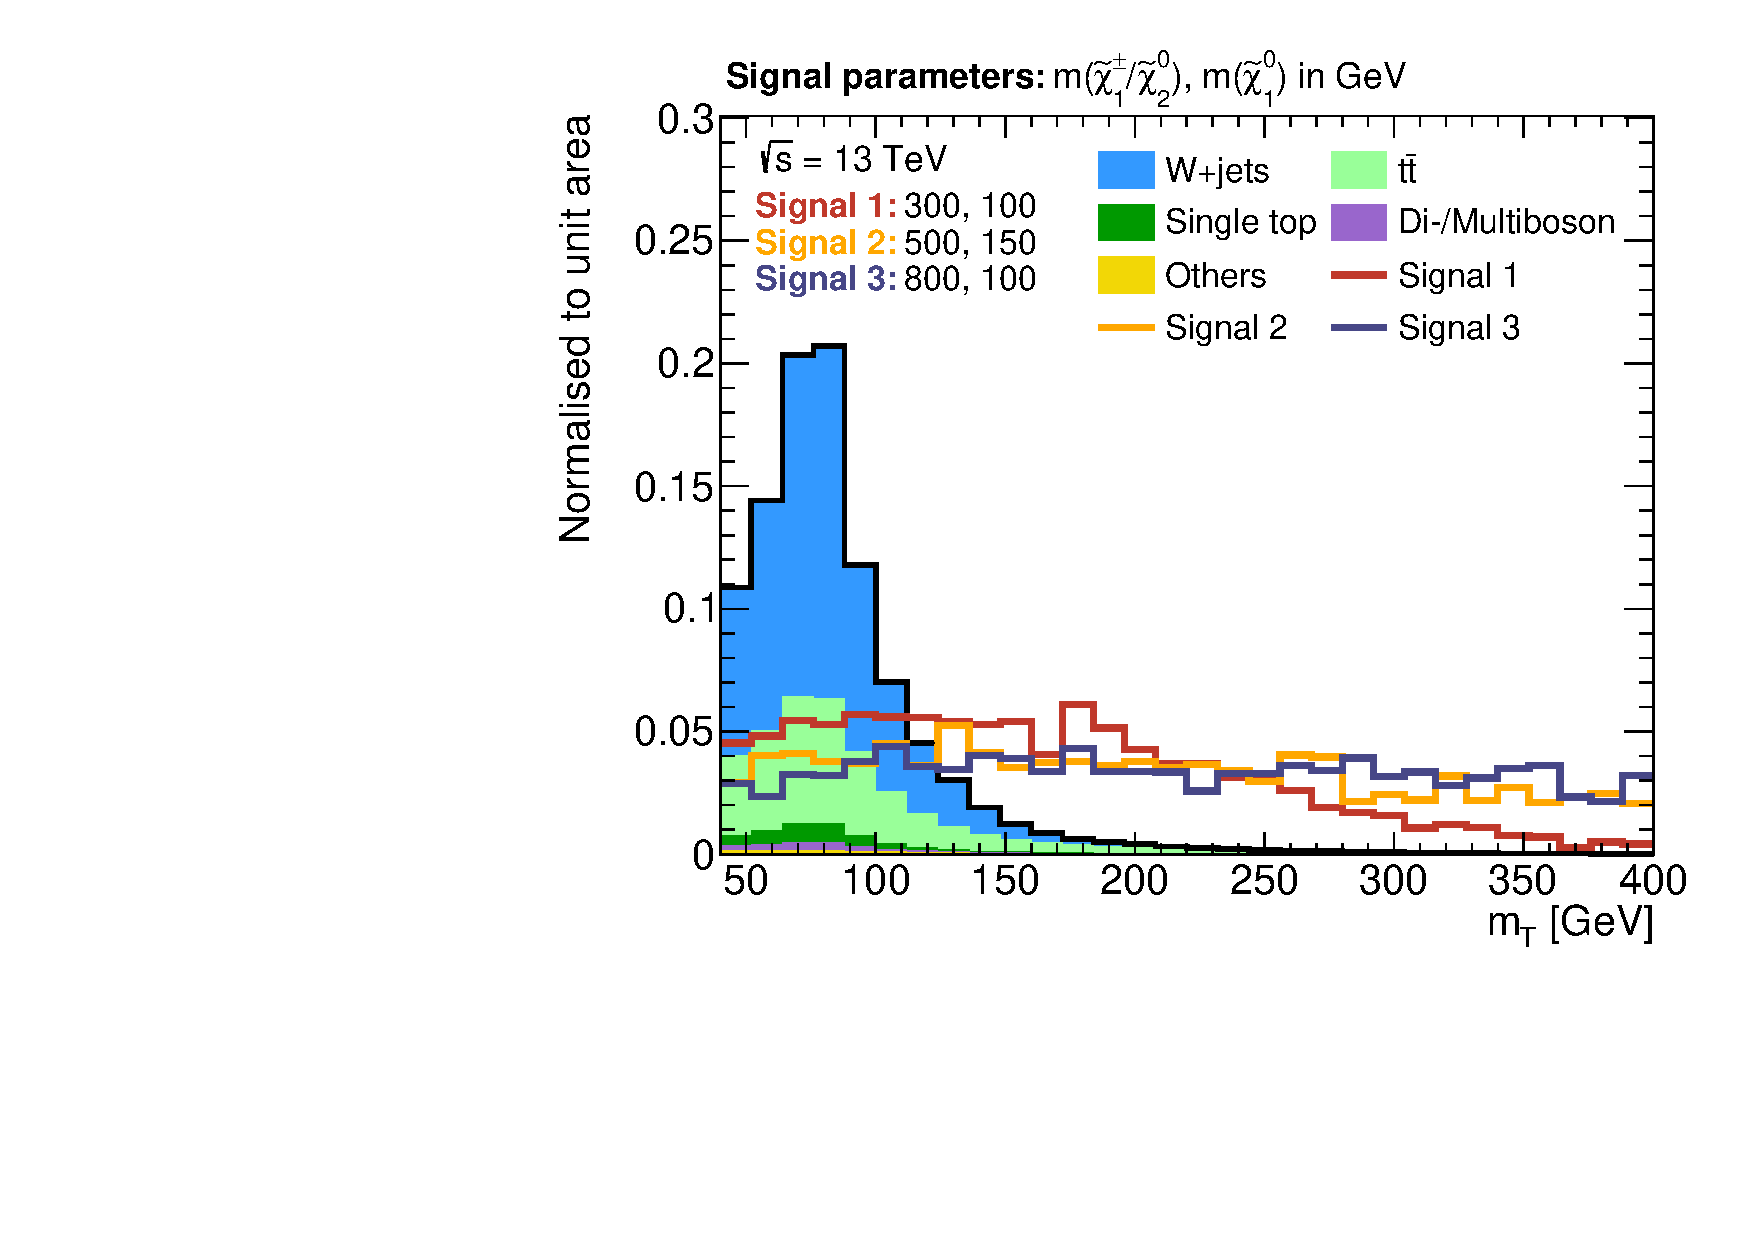
\includegraphics[width=\textwidth]{presel/mt}
		\caption{\label{fig:norm_mt}}
	\end{subfigure}\hfill
	\begin{subfigure}[b]{0.49\linewidth}
		\centering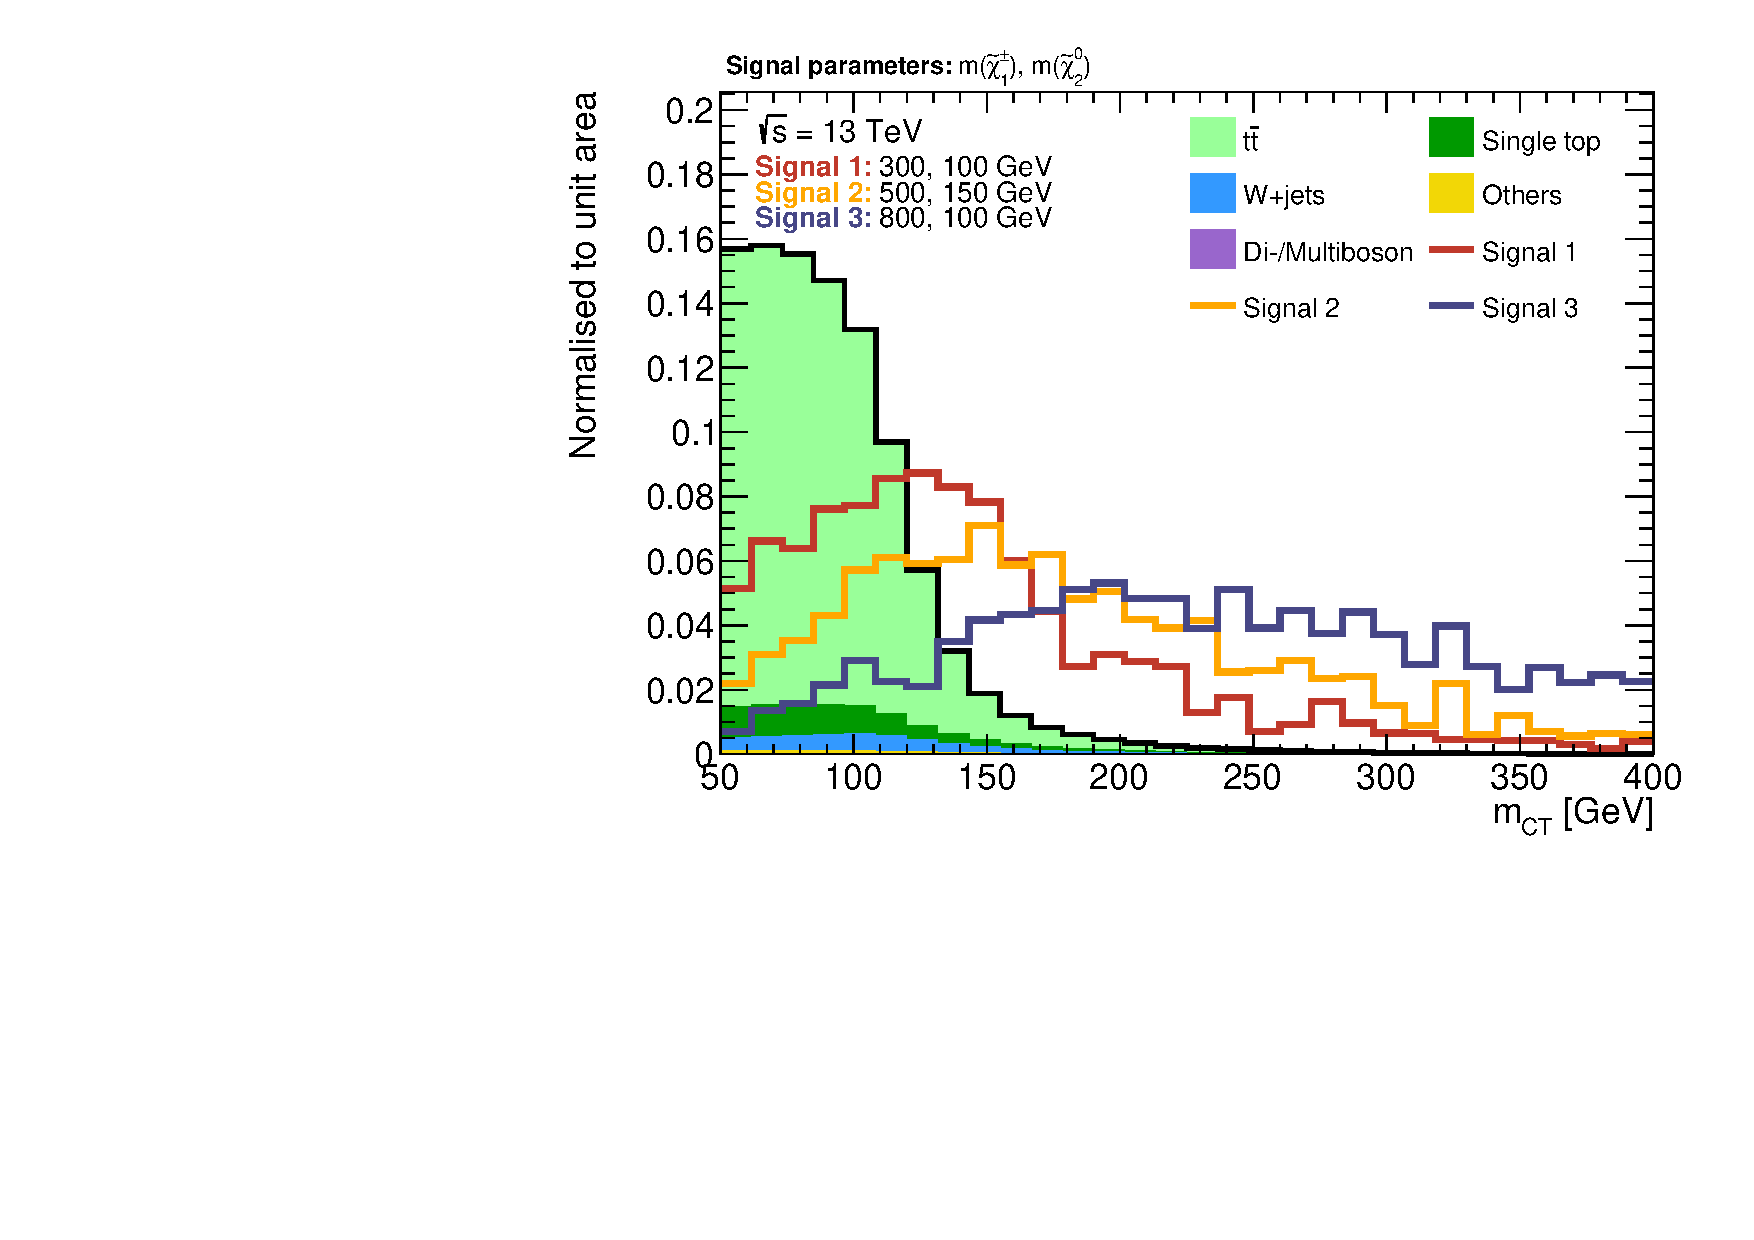
\includegraphics[width=\textwidth]{presel/mct}
		\caption{\label{fig:norm_mct}}
	\end{subfigure}
	\begin{subfigure}[b]{0.49\linewidth}
		\centering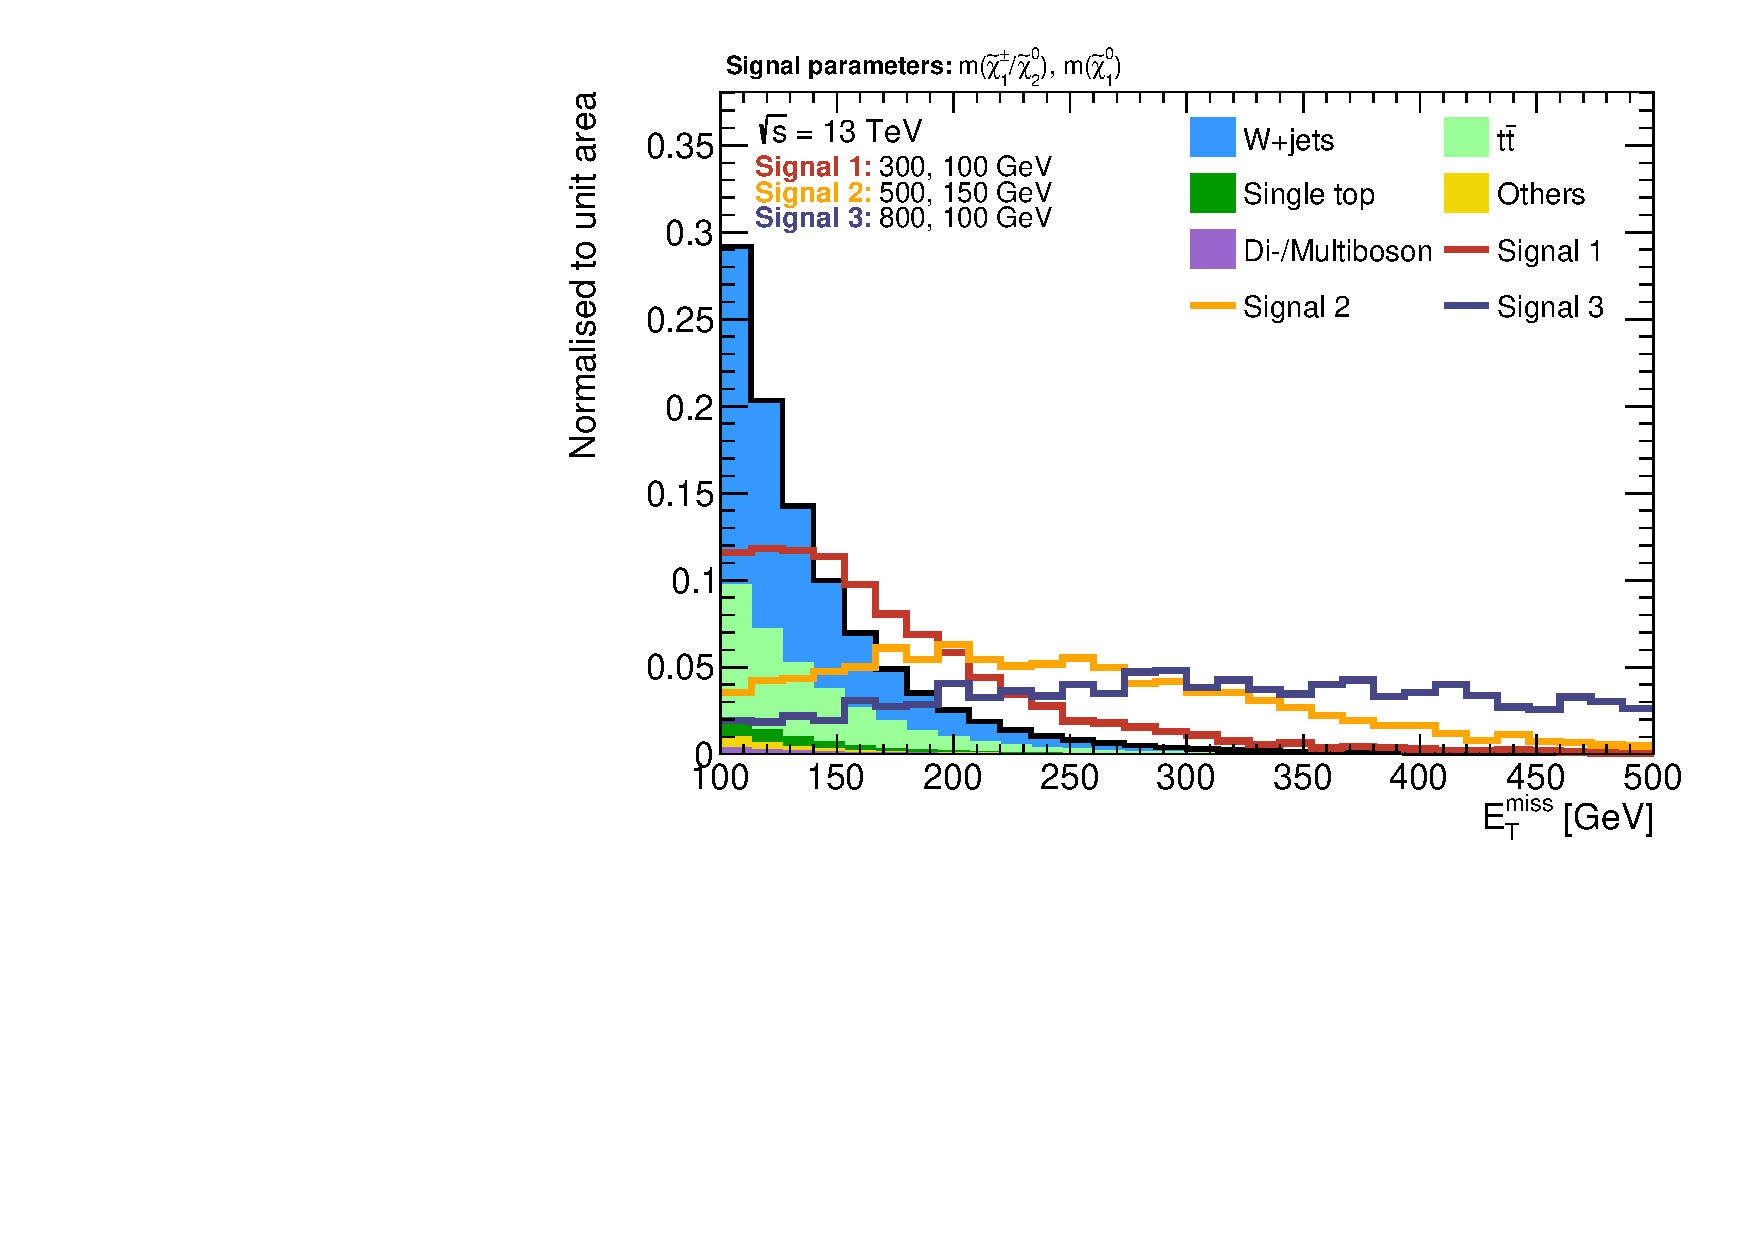
\includegraphics[width=\textwidth]{presel/met}
		\caption{\label{fig:norm_met}}
	\end{subfigure}\hfill
	\begin{subfigure}[b]{0.49\linewidth}
		\centering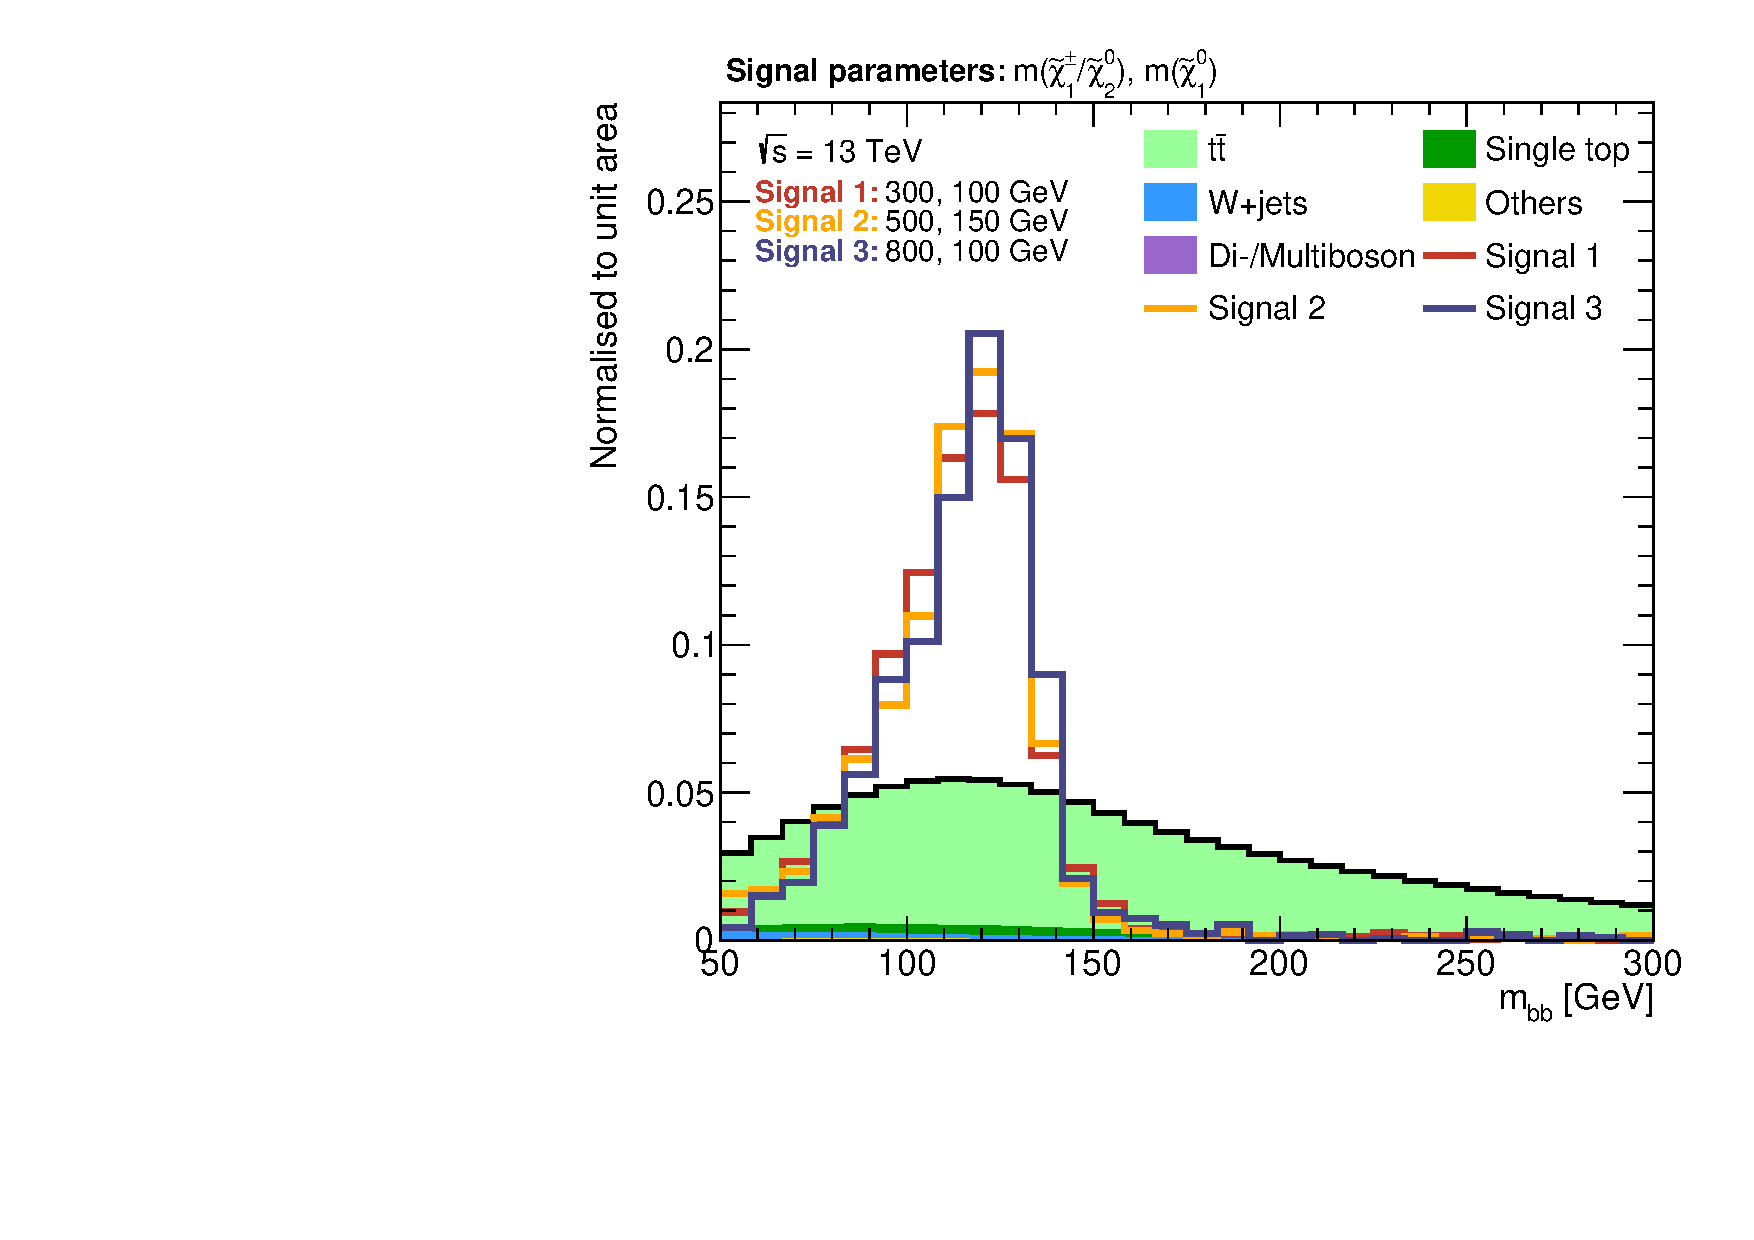
\includegraphics[width=\textwidth]{presel/mbb}
		\caption{\label{fig:norm_mbb}}
	\end{subfigure}
	\begin{subfigure}[b]{0.49\linewidth}
		\centering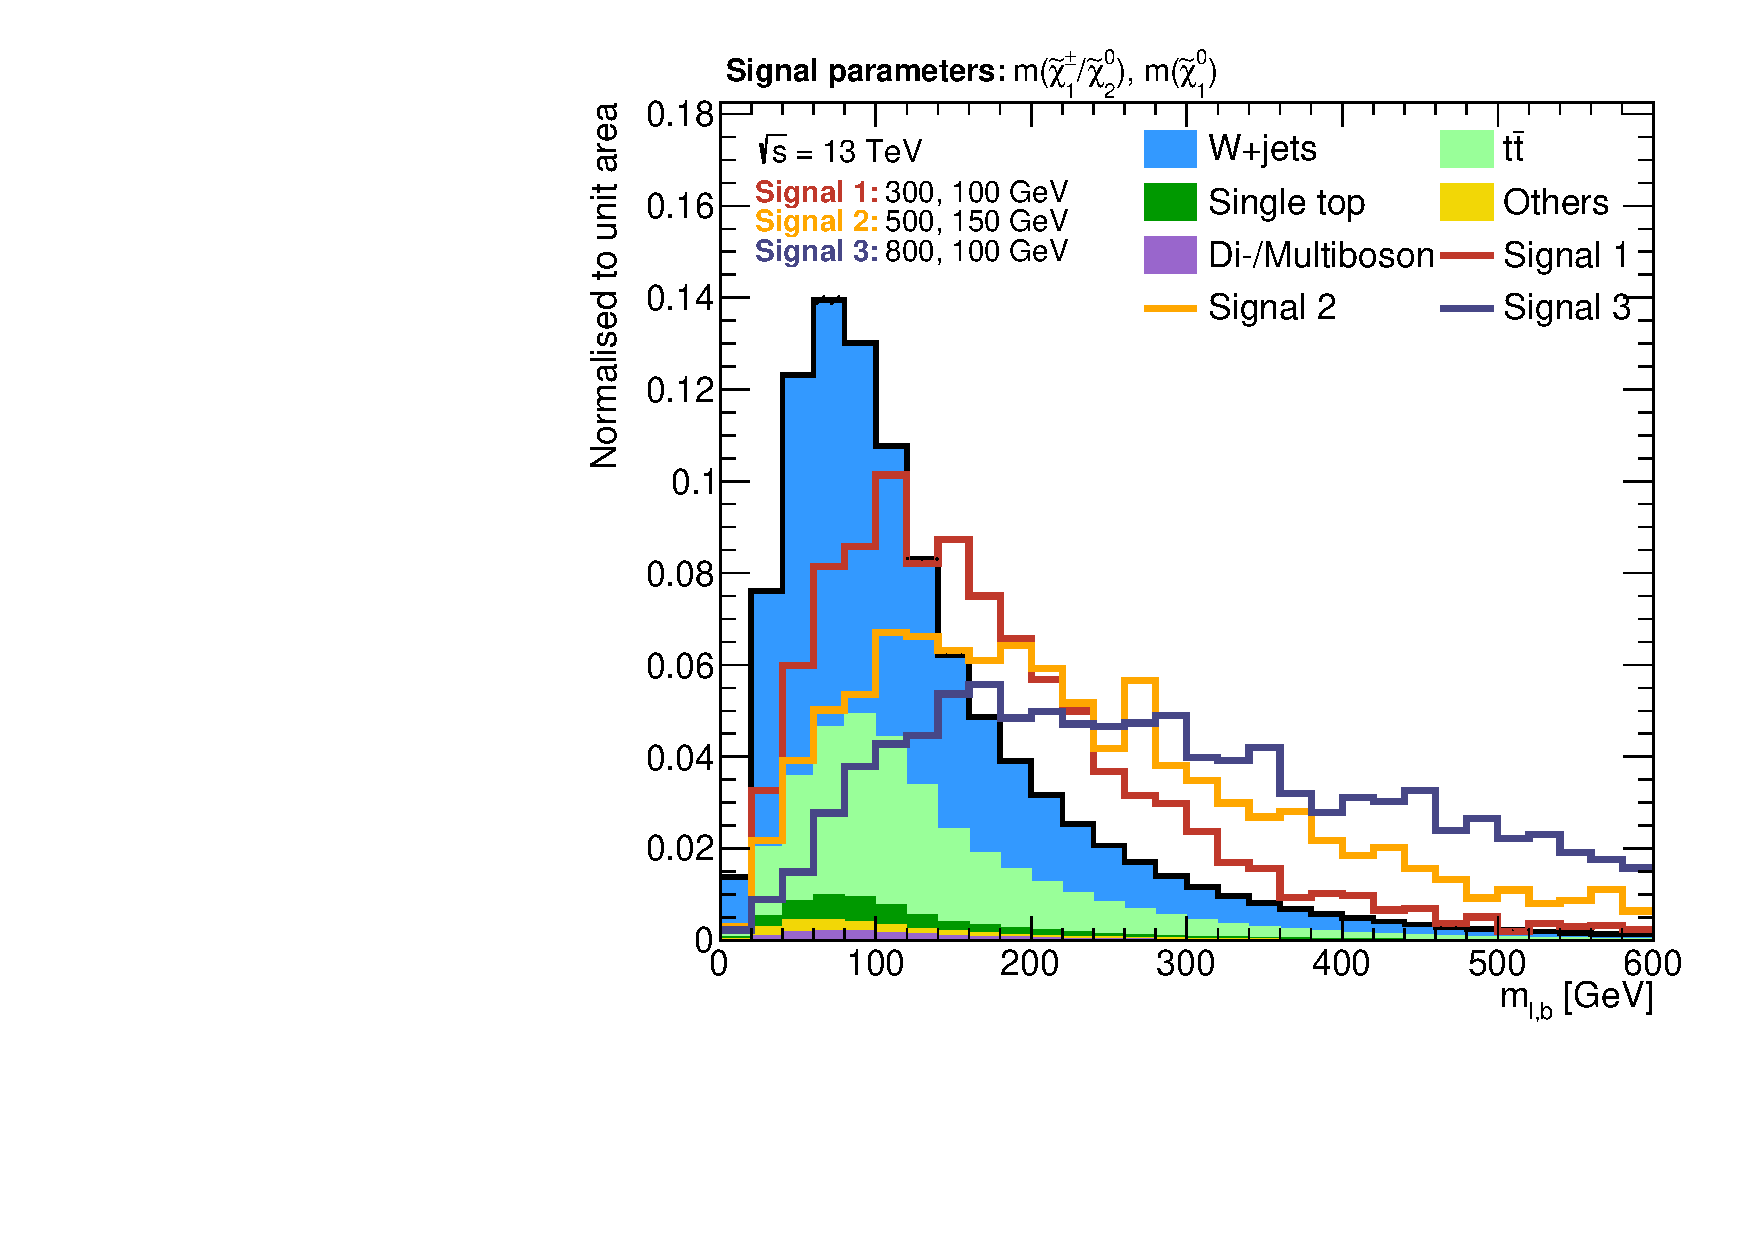
\includegraphics[width=\textwidth]{presel/mlb1}
		\caption{\label{fig:norm_mlb1}}
	\end{subfigure}\hfill
	\begin{subfigure}[b]{0.49\linewidth}
		\centering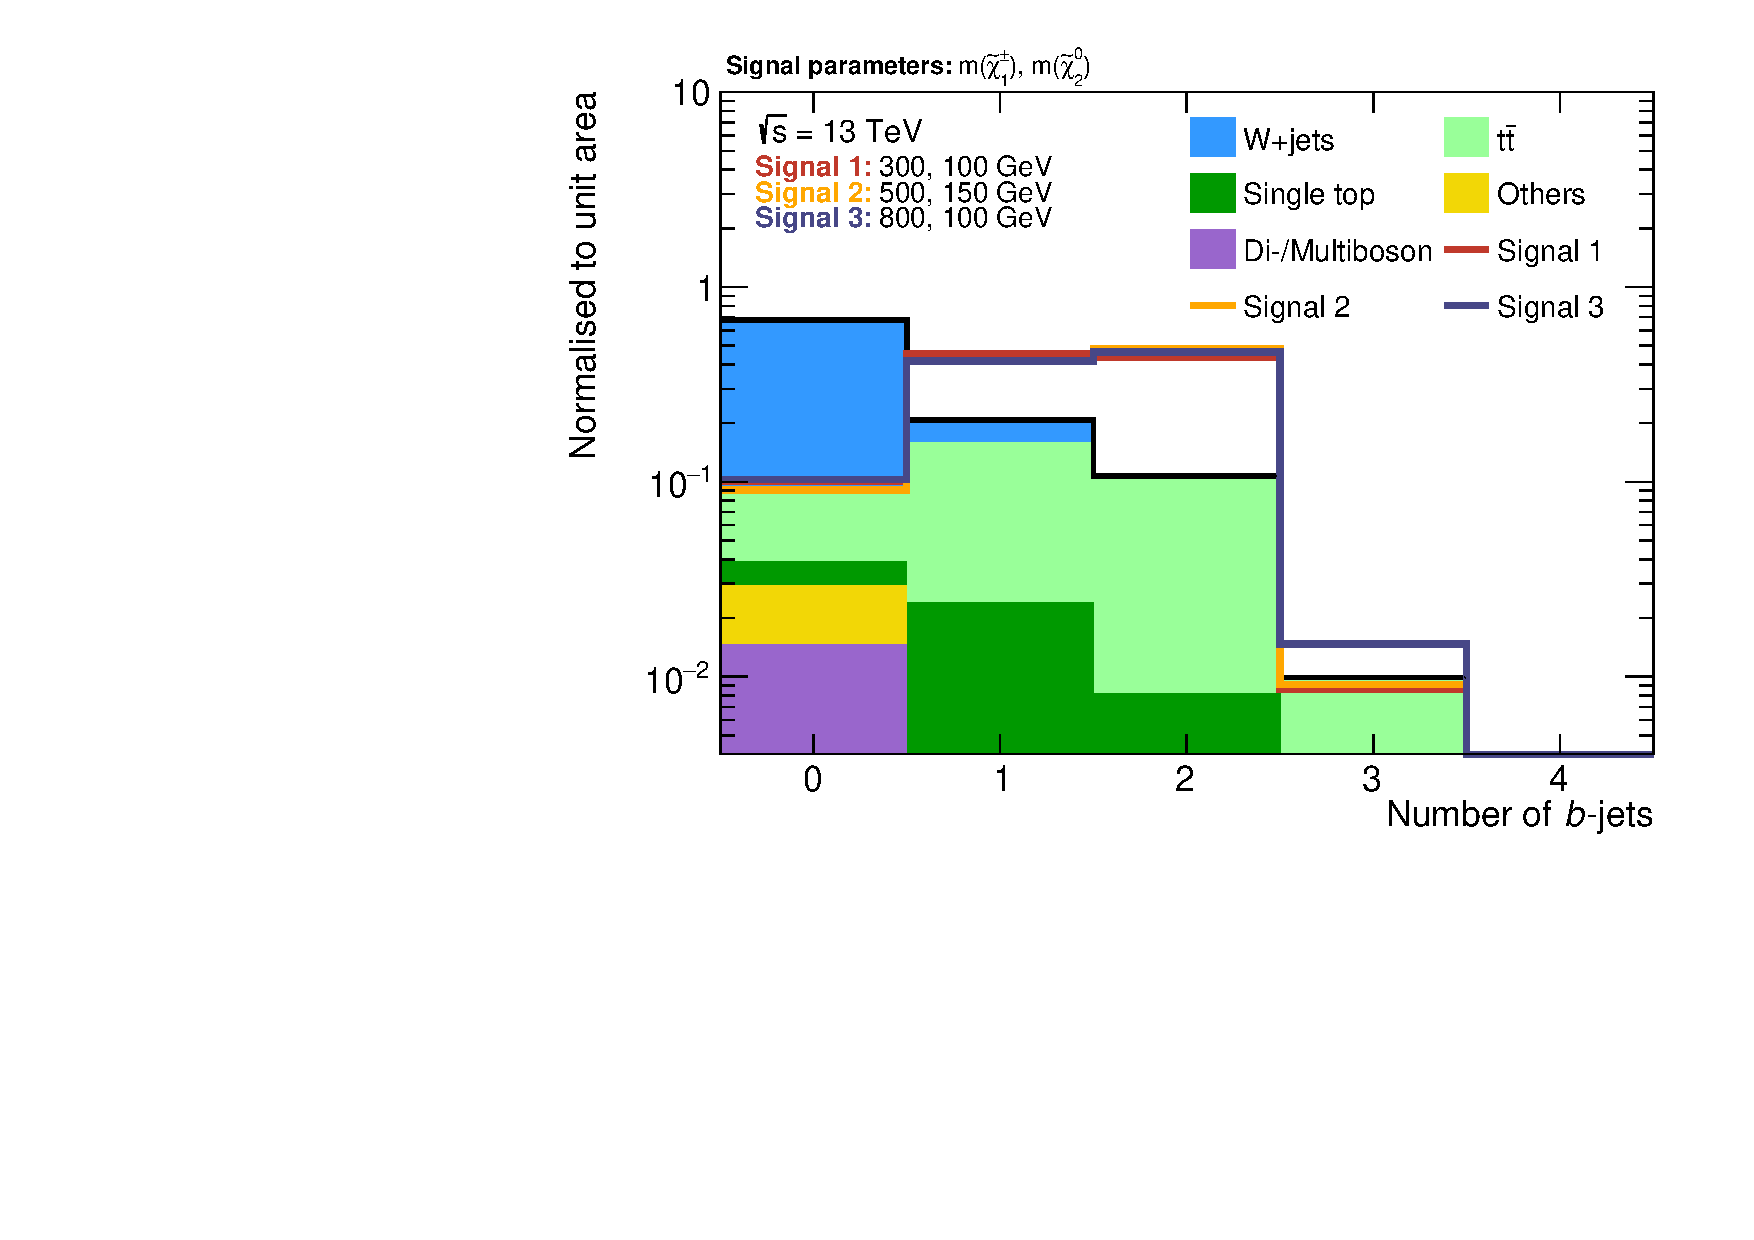
\includegraphics[width=\textwidth]{presel/nBJet}
		\caption{\label{fig:norm_nbjet}}
	\end{subfigure}
	\caption{Distributions of the most important observables used in the analysis. The simulated \gls{sm} backgrounds are stacked on top of each other, and distributions from exemplary signal models with the quoted mass parameters are overlaid. In order to emphasise the shape differences, both total background and signal distributions are normalised to unity. A preselection of a lepton (electron or muon), at least two jets and $\etmiss > \SI{100}{\GeV}$ is applied.}\label{fig:norm_obs}
\end{figure}

\subsubsection{Contransverse mass}

The contransverse mass $\mct$~\cite{Tovey:2008ui} is designed to have a kinematic endpoint for events with pair-produced heavy particles decaying into invisible and visible particles subject to a contra-linear boost. In the following, $\mct$ is defined as
\begin{equation}
	\mct = \sqrt{2\pt^{b_1}\pt^{b_2}(1+\cos\upDelta\phi_{b\hspace{-0.06em}b})},
\end{equation}
where $\pt^{b_1}$ and $\pt^{b_2}$ are the transverse momenta of the two \textit{b}-jets in the final state. Although $\mct$ is invariant under co-linear boosts in the beam direction\footnote{This is by construction the case, as only transverse quantities are used to compute $\mct$.}, it is not invariant under transverse boosts, due to, \eg, \gls{isr} jets. Both the value of $\mct$ and its kinematic endpoint therefore depend on the size and direction of the transverse boost. For this reason, a boost-corrected version of the contransverse mass is used in the following. The correction algorithm is described in detail in \reference\cite{Polesello:2009rn} and uses an estimate of the energy of the upstream pair-produced heavy particles to boost the four-momenta of the visible decay products back into the centre-of-mass frame of the pair-produced particles. The approach provides a conservative value of $\mct$ that is always smaller than the true $\mct$ value measured in the centre-of-mass frame of the pair-produced particles.

For $\ttbar$ events where each top quark decays via $t\rightarrow bW$, the two \textit{b}-jets used for calculating $\mct$ stem from each of the two decay branches of the $\ttbar$ system. It can be shown~\cite{Polesello:2009rn} that, in this case, the boost-corrected contransverse mass has a kinematic endpoint at
\begin{equation}
	\mct^\mathrm{max} = \frac{m^2(t) - m^2(W)}{m(t)} \approx \SI{135}{\GeV}.
\end{equation}
In signal events, the two input \textit{b}-jets originate from the same Higgs boson, and thus $\mct$ does not exhibit a kinematic endpoint, but tends to yield higher values. \Cref{fig:norm_mct} clearly shows the kinematic endpoint for $\ttbar$ backgrounds and further shows that signal distributions result in higher values depending on their mass parameter scales (a behaviour further illustrated in \cref{fig:norm_obs_app}). Similar  as for the transverse mass, varying lower bounds on $\mct$ will be used in \cref{ch:signal_region_optimisation} to define signal regions optimised to different kinematic regimes. 

\subsubsection[Invariant mass of the lepton and leading \textit{b}-jet]{Invariant mass of the lepton and leading $\makemebold{b}$-jet}

The invariant mass of the lepton and the leading \textit{b}-jet, denoted as $\mlb$, is designed to offer high rejection power towards $\ttbar$ and single top processes. In events where the lepton and leading \textit{b}-jet originate from the same top quark decay $t\rightarrow bW \rightarrow b\ell\nu$, the $\mlb$ distribution has a kinematic endpoint at 
\begin{equation}
	\mlb^\mathrm{max} = \sqrt{m^2(t)-m^2(W)} \approx \SI{153}{\GeV} 
\end{equation}
In signal events, the lepton and leading \textit{b}-jet originate from the decay chains of the $\charg$ and $\neutr$, respectively and thus the $\mlb$ distribution depends on the mass scale of the \gls{susy} particles, yielding especially good discriminative power for signal scenarios with high $\charg$/$\neutr$ masses.

\section{Trigger strategy}\label{sec:trigger_strategy}

The trigger strategy of an analysis is crucial to select $pp$ events worth investigating, and typically relies on triggers sensitive to physics objects that are important to the signal scenarios considered. The data used in this analysis has been recorded with $\etmiss$ triggers.
Selecting events with invisible particles is inherently difficult, precisely because these particles do not leave a trace in the detector.
Similar to offline analysis, the trigger algorithms infer the $\etmiss$ from the momenta of the visible particles, but also need to satisfy the stringent event rate constraints set by the high-luminosity environment of the \gls{lhc}.

As described in \cref{sec:trigger}, the \gls{l1} trigger uses only parts of the instrumented regions, a technique that is not well suited for momentum imbalance triggers that rely on a sum of momenta over the full solid angle~\cite{Aad:2020les}.
In the \gls{l1} trigger, dedicated hardware sums the signals from calorimeter cells into \textit{towers} with a granularity matching that of the calorimeter.
Towers of calorimeter cells exceeding a certain threshold are used to generate larger towers with coarser granularity, the $x$ and $y$ projections of which are subsequently summed to get an estimate of $\etmiss$. The tower thresholds are varied to provide stable trigger rates during the different data-taking periods.
The \gls{l1} triggers, used in this analysis, employed a threshold of $\etmiss > \SI{50}{\GeV}$ before feeding passing events to the \gls{hlt} for further analysis. 

Two different types of $\etmiss$ trigger algorithms are used by the \gls{hlt}, one based on jets (\texttt{mht} algorithm), and one implementing local pile-up suppression (\texttt{pufit} algorithm)~\cref{sec:reco_electrons}.
As hadronic jets dominate the visible momentum in most interesting events, using them for $\etmiss$ computation and triggering is well-motivated~\cite{Aad:2020les}.
The \texttt{mht} algorithm was used during the 2015--2016 data taking period and computes the $\etmiss$ from the negative vectorial sum of the transverse momenta of all jets with a transverse momentum $p_\mathrm{T} > \SI{7}{\GeV}$ before calibration~\cite{Aad:2020les}.
The \gls{hlt} jets are reconstructed and calibrated using a similar procedure as for offline analysis, and are thus corrected for pile-up effects~\cite{Aad:2016nrq}.
The \texttt{pufit} algorithm was used during the 2017--2018 data taking period and takes as input topo clusters, formed using the method described in~\cref{sec:reco_electrons}.
The clusters are subsequently combined into $\eta$--$\phi$ patches of size corresponding approximately to that of a jet with $R=0.4$. A correction for pile-up effects, based on the distribution of the energy deposits in the calorimeter, is applied on the clusters.
The \texttt{pufit} algorithm assumes that high $E_\mathrm{T}$ deposits stem from the hard-scatter events while low $E_\mathrm{T}$ deposits originate mostly from pile-up effects~\cite{Aad:2020les}.
The online $\etmiss$ threshold of the triggers increased from $\SI{70}{\GeV}$ to $\SI{110}{\GeV}$ in order to keep the trigger rate more or less stable under the rising instant luminosities during the different data-taking periods.  

Due to resolution effects arising in the combination of the \gls{l1} and \gls{hlt} triggers, and differences in the online reconstruction techniques compared to those used in offline physics analysis, the performance of triggers is in general not a simple step function but consists of a so-called \textit{turn-on curve} with rising efficiency, followed by a \textit{plateau region} with constant efficiency.
In order to achieve the same trigger selection in \gls{mc} as in data, the \gls{mc} events are each assigned a random run number that are distributed according to the respective integrated luminosities of each data taking period.
Using these run numbers, the same triggers used for data-taking during each run can be applied for \gls{mc} events. 

\Cref{fig:trigger_eff} shows the combined $\etmiss$ trigger efficiencies for the electron and muon channels separately.
In the following, an offline requirement of $\etmiss > \SI{240}{\GeV}$ is applied for all analysis regions, selecting events where the $\etmiss$ triggers are fully efficient and no significant difference between \gls{mc} and data is observed.
Thus, no trigger efficiency correction is considered in the following. A statistical uncertainty of 2\% is used to account for the difference between data and \gls{mc} in the trigger plateaus.


\begin{figure}
	\centering
	\begin{subfigure}[b]{0.47\linewidth}
		\centering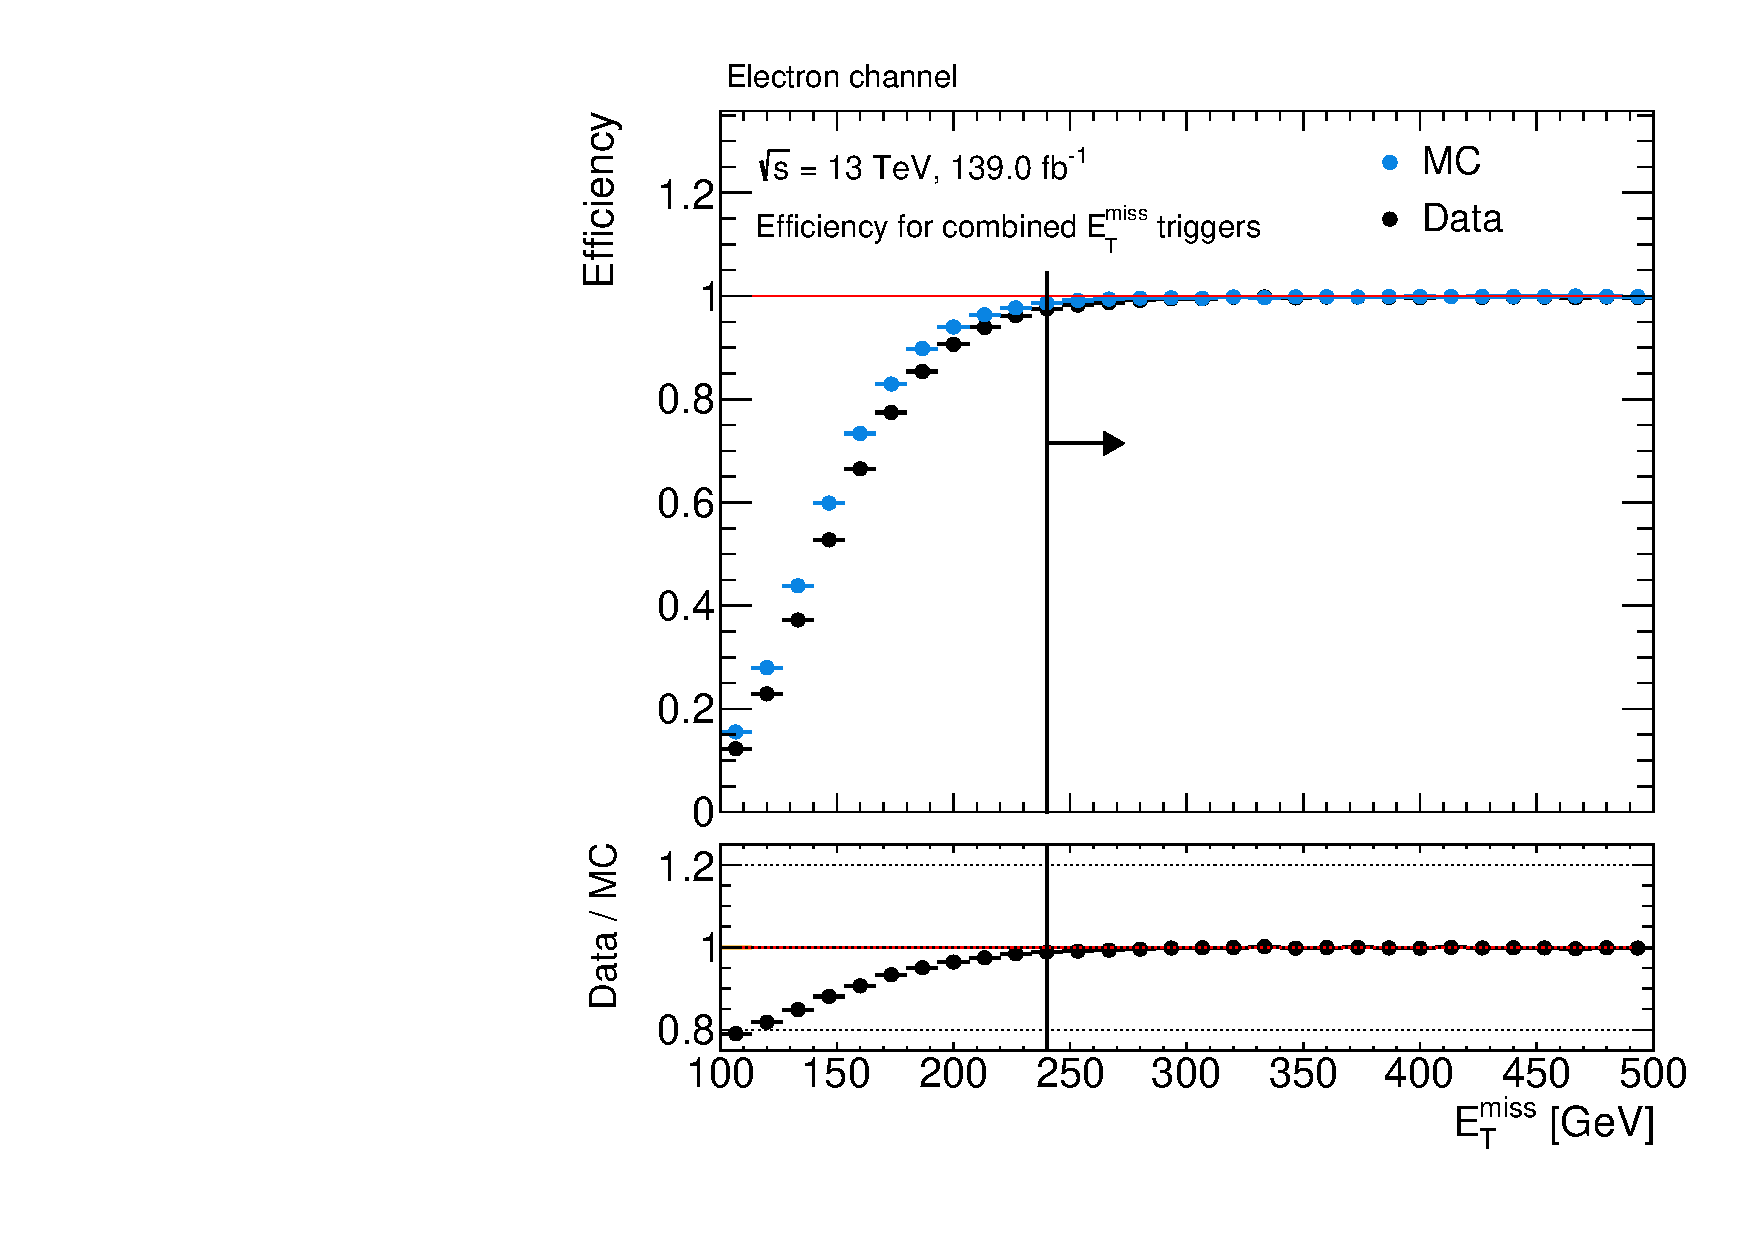
\includegraphics[width=\textwidth]{trigger/met_ele}
		\caption{Electron channel\label{fig:trigger_met_ele}}
	\end{subfigure}\hfill
	\begin{subfigure}[b]{0.47\linewidth}
		\centering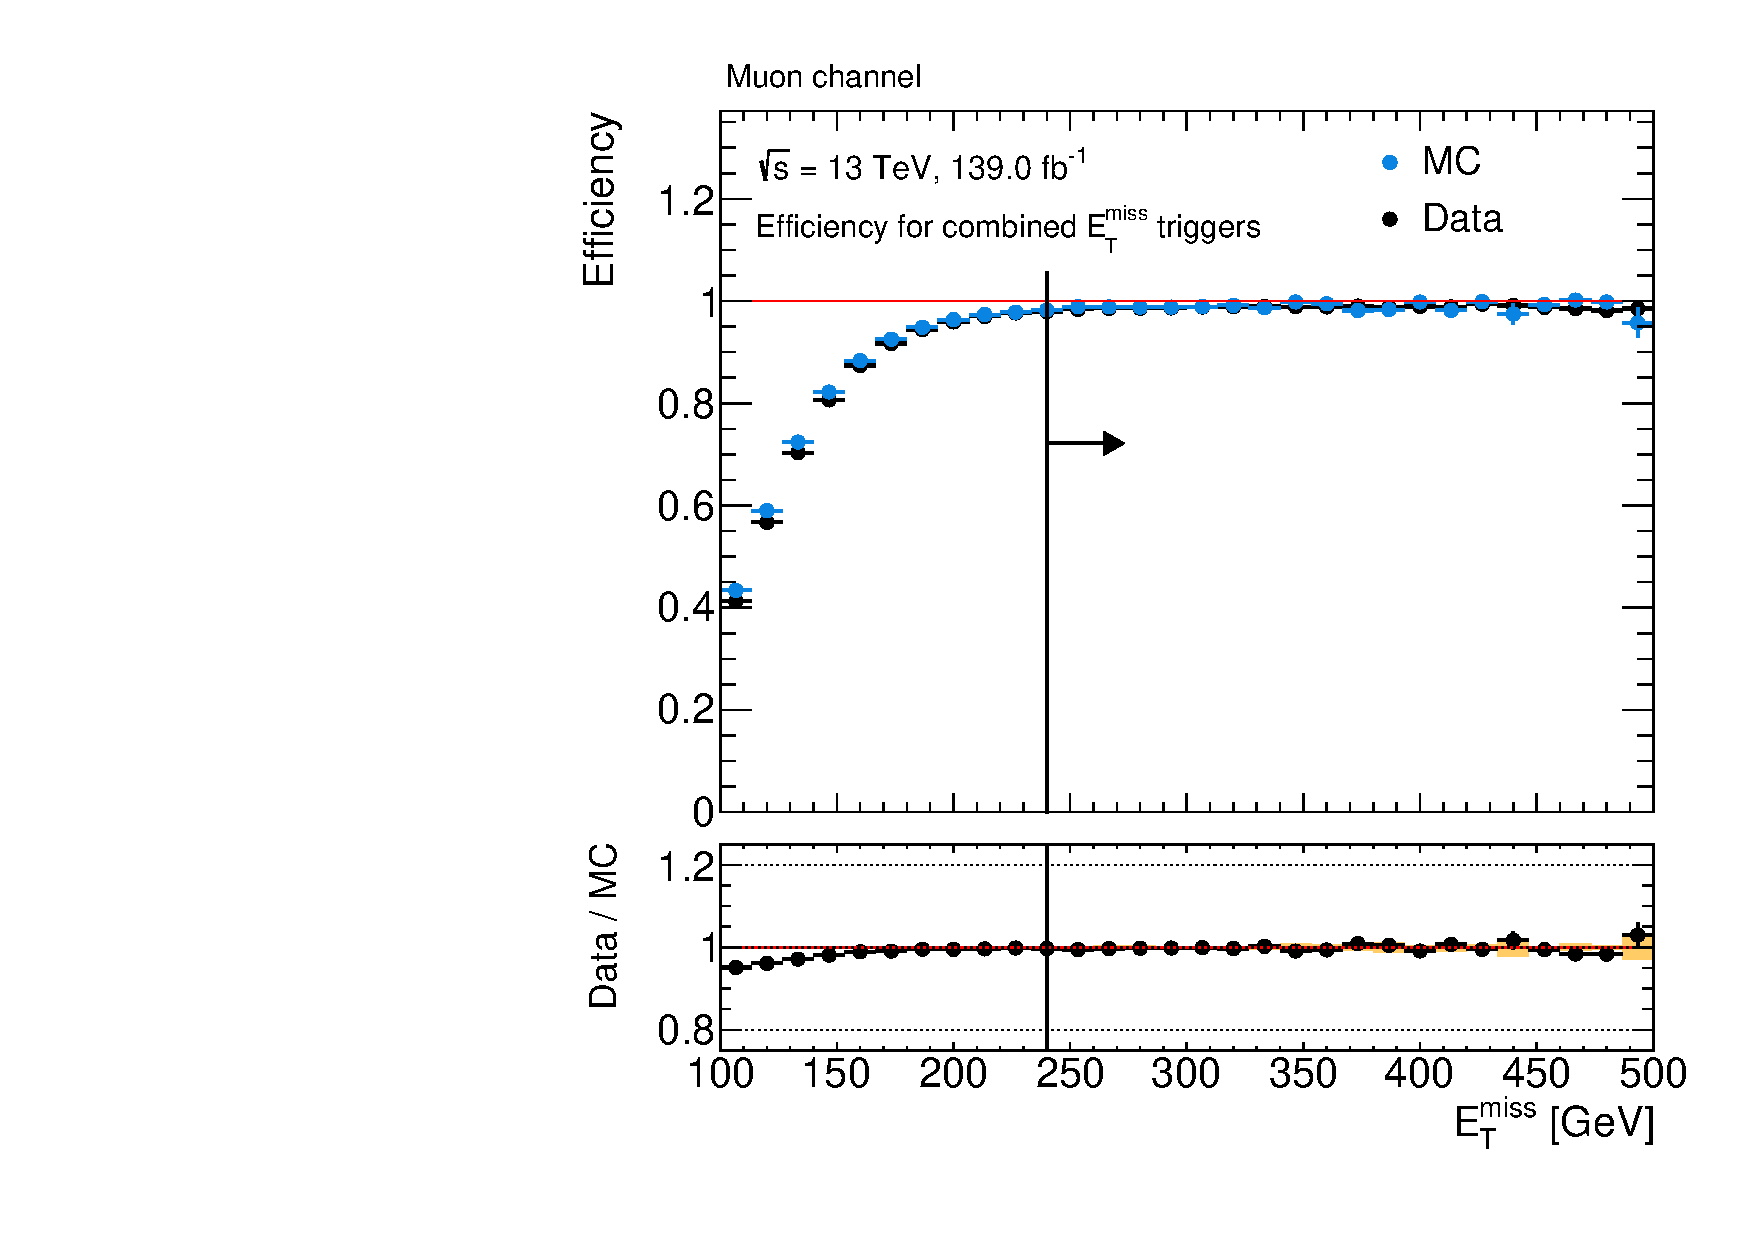
\includegraphics[width=\textwidth]{trigger/met_mu}
		\caption{Muon channel\label{fig:trigger_met_mu}}
	\end{subfigure}
		\caption{Efficiencies of the combined $\etmiss$ triggers in data and \gls{mc} events, triggered by single lepton triggers in the  \subref{fig:trigger_met_ele} electron and \subref{fig:trigger_met_mu} muon channels. A preselection requiring an electron or muon, at least two jets, and $\etmiss > \SI{100}{\GeV}$ is applied on all events. The arrow indicates the offline $\etmiss$ requirement applied on all selections in the analysis.}\label{fig:trigger_eff}
\end{figure}


\section{Event cleaning}

Before being considered for analysis, events need to pass a series of quality requirements.
Data events need to be certified to be good for physics analysis by the ATLAS data quality system~\cite{DAPR-2018-01}, requiring that no transient detector issues have compromised the quality of the data events recorded.
Losses in data quality could happen due to, \eg, high-voltage trips in detector components or noise bursts in the detector electronics~\cite{DAPR-2018-01}.
Only data events are considered where all detector components were flagged as being operational, a process that is performed at the granularity of a \textit{luminosity block}---a time period of roughly $\SI{60}{\second}$ of data-taking where the instantaneous luminosity, detector and trigger configuration are considered to be constant. 

A second series of quality requirements is applied on both data and \gls{mc} events.
To be considered in any subsequent analysis step, events need to contain at least one reconstructed primary vertex with a minimum of two tracks with $\pt > \SI{500}{\MeV}$ associated to it.
Events are discarded where a jet is tagged as originating from a non-collision background process. The \texttt{Loose} working point described in \reference\cite{ATLAS-CONF-2015-029} is used to tag such jets, yielding an efficiency of 99.5\% for jets from $pp$ collision events with $\pt>\SI{20}{\GeV}$.
Similarly, events are rejected if they contain a \textit{bad} muon with a significantly worse than usual momentum resolution that can affect many variables in the entire event and therefore may have sizeable effects on the analysis.
In the following, muons are flagged as \textit{bad} if the relative error on the combined $q/p$ measurement is either larger than $0.2$ or worse than the one from the individual \gls{id} and \gls{ms} track fits.
Events are also rejected if a reconstructed muon is flagged to originate from cosmic radiation, using thresholds on the transverse and longitudinal impact parameters of $d_0 > \SI{0.2}{\milli\meter}$ and $z_0 > \SI{1}{\milli\meter}$ with respect to the primary vertex.



